\documentclass[useAMS,usenatbib]{mn2e}
%\documentclass[twocolumn]{emulateapj}
\usepackage{graphicx,natbib,color,multirow,amsmath}
\voffset=-0.8in

\definecolor{titlecol}{rgb}{0,0,1}
\definecolor{titlecol2}{rgb}{0,0.65,0}
\definecolor{titlecol3}{rgb}{0.99,0.4,0.}

%\definecolor{titledark}{rgb}{0,0,0.8}
%\definecolor{hilit}{rgb}{0,0,1}
%\definecolor{hilitdark}{rgb}{0,0,0.8}
%\font\sbf=cmssbx10 at 32.28pt %big font for headers

\font\nbf=cmssbx10 at 12.28pt %big font for headers

%%%%%%%%%%%%%%%%%%%%%%%%%%%%%%%
%%%% If you want to leave notes in the text feel free to define
%%%% your own colour above and a style below
%%%%%%%%%%%%%%%%%%%%%%%%%%%%%%%
\def\note		{\color{titlecol2} \nbf}
\def\noteb		{\color{titlecol} \nbf}
\def\notebsm	{\color{titlecol}}
\def\notec		{\color{titlecol2} \nbf}
\def\notecsm	{\color{titlecol2}}
\def\notek		{\color{titlecol3} }
\def\builderUC       {} % builder, unconfirmed

%%%%%%%%%%%%%%%%%%%%%%%%%%%%%%%
% For the eventual referee response
\def\changed    {\color{titlecol} }
%\def\changed    {}


%%%%%%%%%%%%%%%%%%%%%%%%%%%%%%%
%  Other stuff I use a lot
\def\oiii		{$\mathrm{\left[ O \textsc{iii}\right] }$}
\def\moiii		{\mathrm{\left[ O \textsc{iii}\right] }}
\def\nii		{$\mathrm{\left[ N \textsc{ii}\right] }$}
\def\mnii		{\mathrm{\left[ N \textsc{ii}\right] }}
\def\sii		{$\mathrm{\left[ S \textsc{ii}\right] }$}
\def\msii		{\mathrm{\left[ S \textsc{ii}\right] }}
\def\galfit     {{\tt GALFIT}}

\def\mmsun	{\rm{M}_{\odot}}
\def\fnobulge    {$f_{\rm no~bulge}$}
\def\mfnobulge {f_{\rm no~bulge}}
\def\fedgeon     {$f_{\rm edge-on}$}
\def\mfedgeon  {f_{\rm edge-on}}
\def\fcnobulge    {$f_{\rm confirmed~no~bulge}$}
\def\mfcnobulge {f_{\rm confirmed~no~bulge}}

\def\kappamean {$\overline{\kappa}$}
\def\mkappamean {\overline{\kappa}}
\def\stellarity   {{\tt CLASS\_STAR}}


%\def\lesssim{\mathrel{\hbox{\rlap{\hbox{\lower5pt\hbox{$\sim$}}}\hbox{$<$}}}}
%\def\gtrsim{\mathrel{\hbox{\rlap{\hbox{\lower5pt\hbox{$\sim$}}}\hbox{$>$}}}}
%new defs of lesssim gtrsim that I think look better
\def\lesssim{\mathrel{\hbox{\rlap{\hbox{\lower3pt\hbox{$\sim$}}}\hbox{\raise2pt\hbox{$<$}}}}}
\def\gtrsim{\mathrel{\hbox{\rlap{\hbox{\lower3pt\hbox{$\sim$}}}\hbox{\raise2pt\hbox{$>$}}}}}


\newcommand\nodata{ ~$\cdots$~ }




\begin{document}

\title[Galaxy Zoo: CANDELS Data Release]{Galaxy Zoo: Detailed Morphological Classifications for 48,000 galaxies from CANDELS\thanks{This publication has been made possible by the participation of more than 95,000 volunteers in the Galaxy Zoo project. The contributions of the more than $40,000$ of those who registered a username with Galaxy Zoo are
individually acknowledged at http://authors.galaxyzoo.org/ .} } 

\author[Simmons et al.]{\parbox[t]{16cm}{B. D. Simmons$^{1}\thanks{E-mail: brooke.simmons@astro.ox.ac.uk}$, {\notebsm and a \emph{lot} of other people to be named later}
%Chris Lintott$^{1,3}$, 
%Kyle W. Willett$^{5}$, 
%Karen L. Masters$^{2,4}$, 
%Robert C. Nichol$^{2,4}$, 
%William C. Keel$^{6}$, 
%Thomas Melvin$^{2}$, 
%R. J. Smethurst$^{1}$, 
%Edmond Cheung$^{7}$, 
%Kevin Schawinski$^{8}$, 
%Michael Rutkowski$^{5}$,
%Jeyhan S. Kartaltepe$^{9,}$\footnote{Hubble Fellow}, 
%Kevin R. V. Casteels$^{11}$, 
%Christopher J. Conselice$^{12}$,
%Omar Almaini$^{12}$, 
%Henry C. Ferguson$^{13}$,
%Lucy Fortson$^{5}$, 
%William Hartley$^{12,8}$, 
%Dale Kocevski$^{14}$,
%Anton M. Koekemoer$^{13}$,
%Daniel H. McIntosh$^{15}$,
%Alice Mortlock$^{12}$, 
%{\builderUC Jeffrey A. Newman$^{16}$,}
%Jamie Ownsworth$^{12}$, 
%Steven Bamford$^{12}$,
%{\builderUC Tomas Dahlen$^{13}$,} 
%{\builderUC Sandra M. Faber$^{17}$,}
%{\builderUC Steven L. Finkelstein$^{18}$,} 
%{\builderUC Adriano Fontana$^{19}$,}
%{\builderUC Audrey Galametz$^{19}$,}
%N. A. Grogin$^{13}$,
%{\builderUC Ruth Gr\"utzbauch$^{12, 20}$,} 
%{\builderUC Yicheng Guo$^{17}$,}
%{\builderUC Boris H\"au\ss ler$^{12,21,1}$,}
%Kian Jek$^{22}$,
%Sugata Kaviraj$^{21}$,
%Ray A. Lucas$^{13}$,
%{\builderUC Michael Peth$^{23}$,}
%{\builderUC Mara Salvato$^{24}$,} 
%{\builderUC Tommy Wiklind$^{25}$,} 
%{\builderUC Stijn Wuyts$^{24}$}
%
\vspace{0.1in} }\\
$^{1}$Oxford Astrophysics, Denys Wilkinson Building, Keble Road, Oxford OX1 3RH, UK\\
%$^{2}$Institute of Cosmology \& Gravitation, University of Portsmouth, Dennis Sciama Building, Portsmouth PO1 3FX, UK\\
%$^{3}$Adler Planetarium, 1300 S. Lake Shore Drive, Chicago, IL 60605, USA\\
%$^{4}$SEPnet,\thanks{www.sepnet.ac.uk} South East Physics Network\\
%$^{5}$School of Physics and Astronomy, University of Minnesota, 116 Church St. SE, Minneapolis, MN 55455, USA\\
%$^{6}$Department of Physics and Astronomy, University of Alabama, Box 870324, Tuscaloosa, AL 35487, USA\\
%$^{7}$Department of Astronomy and Astrophysics, 1156 High Street, University of California, Santa Cruz, CA 95064, USA\\
%$^{8}$Institute for Astronomy, ETH Z\"urich, Wolfgang-Pauli-Strasse 27, CH-8093 Z\"urich, Switzerland\\
%$^{9}$National Optical Astronomy Observatory, 950 N. Cherry Ave., Tucson, AZ, 85719, USA\\
%$^{10}$Department of Astronomy, University of Michigan, Ann Arbor, MI 48104, USA\\
%$^{11}$Institut de Cincies del Cosmos. Universitat de Barcelona (UB-IEEC), Mart i Franqus 1, E-08028 Barcelona, Spain\\
%$^{12}$School of Physics \& Astronomy, University of Nottingham, Nottingham NG7 2RD\\
%$^{13}$Space Telescope Science Institute, 3700 San Martin Drive, Baltimore, MD 21218\\
%$^{14}$Department of Physics and Astronomy, University of Kentucky, Lexington, KY 40506, USA\\
%$^{15}$Department of Physics, University of Missouri-Kansas City, 5110 Rockhill Road, Kansas City, MO 64110, USA\\
%$^{16}$Department of Physics and Astronomy \& PITT PACC, University of Pittsburgh, Pittsburgh, PA 15217, USA\\
%$^{17}$UC Observatories/Lick Observatory and Department of Astronomy and Astrophysics, University of California, Santa Cruz, CA 95064, USA\\
%$^{18}$Department of Astronomy, The University of Texas at Austin, Austin, TX 78712, USA\\
%$^{19}$INAF-Osservatorio Astronomico di Roma, Via Frascati 33, I-00040, Monteporzio, Italy\\
%$^{20}$Centre for Astronomy and Astrophysics, University of Lisbon, P-1349-018 Lisbon, Portugal\\
%$^{21}$Centre for Astrophysics Research, University of Hertfordshire, College Lane, Hatfield AL10 9AB, UK\\
%$^{22}$Galaxy Zoo Volunteer\\
%$^{23}$Department of Physics and Astronomy, The Johns Hopkins University, Baltimore, MD 21218, USA\\
%$^{24}$Max-Planck-Institut f{\"u}r extraterrestrische Physik, Giessenbachstrasse 1, D�85748 Garching bei M{\"u}nchen, Germany\\
%$^{25}$European Southern Observatory/Joint ALMA Observatory, 3107 Alonso de Cordova, Santiago, Chile\\
   }

\maketitle
  
\label{firstpage}
  
%\clearpage

\begin{abstract}

We present quantified visual morphologies of approximately 48,000 galaxies having $z \lesssim 3$, using galaxies observed in three \emph{Hubble Space Telescope} legacy fields by the Cosmic And Near-infrared Deep Extragalactic Legacy Survey (CANDELS) and classified by participants in the Galaxy Zoo project. Each galaxy received an average of 43 independent classifications, which we combine into detailed morphological information on galaxy features such as clumpiness, bar instabilities, spiral structure, and merger and tidal signatures. We apply a consensus-based classifier weighting method that preserves classifier independence while effectively down-weighting significantly errant classifications. After analysing the effect of varying image depth on reported classifications, we also provide depth-corrected classifications to preserve the information in the deepest observations and also enable the use of classifications at comparable depths across the full survey. Comparing the Galaxy Zoo classifications to previous human and machine classifications of the same galaxies shows very good agreement; in some cases the high number of independent classifications provided by Galaxy Zoo provides an advantage in selecting galaxies with a particular morphological profile, while in others the combination of Galaxy Zoo with other classifications is a more promising approach than using any one method alone. We combine the Galaxy Zoo classifications of ``smooth'' galaxies with parametric morphologies to select a sample of featureless disks at $1 \leq z \leq 2$, which may represent a dynamically warmer progenitor population to the settled disk galaxies seen at later epochs.


  \end{abstract}
  
  \begin{keywords}
  
  galaxies: general 
  --- 
  galaxies: evolution
  --- 
  galaxies: morphology %not actually a keyword 
  --- 
  galaxies: structure
  
  \end{keywords}

%%%%%%%%%%%%%%%%%%%%%%%%%%%%%%%%%%%%%%%%%%%%%%
%
%  
\section{Introduction}
%
%
%%%%%%%%%%%%%%%%%%%%%%%%%%%%%%%%%%%%%%%%%%%%%%

This paper presents morphological classifications of nearly $50,000$ galaxies imaged in the Cosmic And Near-infrared Deep Extragalactic Legacy Survey \citep[CANDELS;][]{grogin11,koekemoer11} measured by the Galaxy Zoo{\footnote{zoo4.galaxyzoo.org}} project \citep{lintott08}. Over 95,000 volunteers have contributed over 2,000,000 detailed galaxy classifications to this effort. We combine, on average, 43 independent classifications of each galaxy to produce detailed, quantitative morphological descriptions of these distant galaxies along many physical axes of interest. 

The shape and appearance of a galaxy trace the underlying physical processes that have formed it and continue to influence its evolution. For example, the signatures of past merger events \citep[from $z \sim 2$ onwards;][]{martig12} are visible even at $z = 0$ in the form of a galactic bulge; the strength of the bulge is tied to the strength of the merger, as indeed the lack of a bulge indicates a lack of significant mergers \citep[e.g.,][]{kormendy10}. Likewise, other morphological features are tied to disk instabilities and resonances \citep[e.g.,][]{kormendy04,b_elmegreen08,donghia13}, and orbital changes from the disruptive \citep[mergers; e.g.,][]{darg10a,darg10b,lotz08a,lotz08b} to the relatively subtle \citep[e.g., bars,][]{athanassoula92b,sellwood93,athanassoula05,athanassoula13,simmons14}. Furthermore, combination of morphological parameters with other measures, such as environment, color, mass and star formation histories \citep[e.g.][]{bamford09,tojeiro07,schawinski14,smethurst15}, can provide more insight than either alone.

Morphological measures have a long history in astronomy \citep[e.g.,][]{hubble26,devaucouleurs,devaucouleurs59,sandage61,vandenbergh76,abraham96c,nair10}. The computerized era of astrophysics has brought with it a number of automated morphological classification techniques. Some use multiple parameters to characterise a galaxy's distribution of light \citep{sersic68,odewahn02}, while others adopt a non-parametric approach, each reducing a galaxy to one number \citep[and often used in combination; e.g.][]{abraham94, conselice03, lotz04a}. Both types of analyses lend themselves relatively well to large-scale processing of images from galaxy surveys \citep[e.g.][]{simard02,scarlata07,simard09,griffith12,lackner12,lackner13} and provide a uniform quantitative set of measures. Modern machine learning techniques, with appropriate training, are also applicable to large data sets \citep{huertascompany08,huertascompany15,dieleman15}.

However, no computer has yet exceeded the human brain's capacity for pattern detection and serendipitous discovery. Visual morphologies remain among the most nuanced and powerful measures of galaxy structure. Galaxy Zoo combines the strengths of both visual and computer-driven approaches, using the Internet to collect more independent and complete visual classifications than any group of astronomers is realistically capable of and combining these classifications via tested and proven techniques.

Since 2007, Galaxy Zoo has been a unique resource of quantitative and statistically robust visual galaxy morphologies. Prior to Galaxy Zoo CANDELS, three Galaxy Zoo projects have collected morphologies for over $1,000,000$ galaxies using the largest surveys to date to $z \sim 1$. These projects have been and continue to be extremely scientifically productive, both for the project team \citep[e.g.,][]{keel15,galloway15,willett15} and for the larger scientific community \citep[e.g.][]{amorin10,finkelman12,robaina12,combes13,joachimi15,zhang15,lopezcorredoira15}.

Here we present the Galaxy Zoo visual morphologies of $49,555$ galaxies imaged by the largest near-infrared \emph{Hubble Space Telescope (HST)} survey to date, CANDELS, which images galaxies at rest-frame optical wavelengths to $z \approx 2.7$. 

In Section \ref{sec:data} we describe the observational data and the preparation of CANDELS images for use in Galaxy Zoo. In Section \ref{sec:classifications} we detail the collection of morphological classifications and the method of weighting and combining independent classifications for each galaxy. Section \ref{sec:comparison} compares Galaxy Zoo classifications to other morphological measurements. In Section \ref{sec:result} we show an example result using the classifications, and in Section \ref{sec:summary} we summarize. Throughout
this paper we use the AB magnitude system, and where necessary we adopt a cosmology consistent with $\Lambda$CDM, with $H_{\rm 0}=70~{\rm
km~s^{-1}}$Mpc$^{\rm -1}$, $\Omega_{\rm m}=0.3$ and $\Omega_{\rm \Lambda}=0.7$ \citep{bennett13}.




%%%%%%%%%%%%%%%%%%%%%%%%%%%%%%%%%%%%%%%%%%%%%%
%
%
\section{Observational Data}\label{sec:data}
%
%
%%%%%%%%%%%%%%%%%%%%%%%%%%%%%%%%%%%%%%%%%%%%%%

\subsection{Images}\label{sec:images}

% Edited by CJL
The Cosmic Assembly Near-infrared Extragalactic Legacy Survey \citep[CANDELS;][]{grogin11,koekemoer11} is an \emph{HST} Treasury programme combining optical and near-infrared imaging from the Advanced Camera for Surveys (ACS) and Wide Field Camera 3 (infrared channel; WFC3/IR), providing an unprecedented opportunity to study galaxy structure and evolution across a range of redshifts. CANDELS covers the area included in five fields which had been targeted for previous studies {(GOODS-North and -South, \citeauthor{giavalisco04} \citeyear{giavalisco04}; EGS, \citeauthor{davis07} \citeyear{davis07}; UDS, \citeauthor{lawrence07} \citeyear{lawrence07}, \citeauthor{cirasuolo07} \citeyear{cirasuolo07}; and COSMOS, \citeauthor{scoville07} \citeyear{scoville07}), divided into `deep' and `wide' fields. Each of the wide fields (UDS, COSMOS, EGS and flanking fields to the GOODS-S and GOODS-N deep fields) are imaged over 2 orbits in WFC3/IR, split in a 2:1 ratio between filters F160W and F125W respectively, with parallel exposures made in F606W and F814W using ACS. Each of the deep fields (corresponding to those targeted by GOODS-S and GOODS-N) are imaged over at least 4 orbits each in both the F160W and F125W filters and 3 orbits in the F105W filter, with ACS exposures in F606W and F814W in parallel. These data are reduced and combined to produce a single mosaic for each field in each band, with drizzled resolutions of $0.03^{\prime\prime}$ and $0.06^{\prime\prime}$ per pixel for ACS and WFC3/IR, respectively \citep{koekemoer11}.

The 4th release of Galaxy Zoo included all detections with $H \leq 25.5$ from COSMOS, GOODS-South and UDS, comprising 49,555 unique images. These were shown to visitors to the website galaxyzoo.org starting on the 10th of September, 2012. The images shown to the public are colour composites of ACS $I$ ($F814W$), WFC3 $J$ ($F125W$), and WFC3 $H$ ($F160W$) filters for the blue, green and red channels, respectively. Previous iterations of Galaxy Zoo \citep{lintott08} have shown that the effect of showing colour images (rather than monochrome or single filter images) on classifications is small, but doing so greatly increases classifier engagement. The angular sizes of the images in different filters are matched, and the native point-spread functions (PSFs) are used. The images are combined with an asinh stretch \citep[described in detail in][]{lupton04} with a non-linearity value of {\notebsm 3.0}, chosen as a compromise between the need to show clear features across a wide dynamic range. 

Sources in the dataset vary greatly in size and surface brightness, and a single set of values for channel scalings is not adequate to capture the variety of features across the images. We therefore use a variable scaling based on the {\notebsm magnitude and size} of each target source. For each image the R, G, and B channels have a fixed ratio of {\notebsm [not sure; must get this from Jeyhan]}, and the multiplier can vary between {\notebsm A and B}. Figure \ref{fig:imageexamples} shows examples of these colour composites across a wide range of source fluxes and sizes. 

Each colour image is 424 pixels square. The angular size of the image varies, such that the colour image encompasses at least {\notebsm 3 times the 80\% flux radius of the target source}, with a minimum screen-to-WFC3 zoom ratio of {\notebsm 1:10} and a maximum ratio of {\notebsm 3:1}. The Galaxy Zoo interface loads the normal colour images by default, and the classifier may choose to display an inverted colour image, but may not otherwise change the image scaling or size within the software while performing the classification; this design ensures a consistent set of classifications which can be combined as described below.



\subsection{Photometry}

Selection of galaxies to include in Galaxy Zoo CANDELS was based on preliminary photometry of the ACS and WFC3 images, computed using Source Extractor \citep{bertin96}. As described in Section \ref{sec:images}, the sample was selected using $H \leq 25.5$~mag. 

Subsequent analysis has produced more refined photometry in each field (GOODS-S, \citeauthor{guo13} \citeyear{guo13}; UDS, \citeauthor{galametz13} \citeyear{galametz13}; COSMOS, M. Peth et al., in preparation). In particular, an adapted form of Source Extractor has been used to more cleanly determine backgrounds and provide improved flux measurements. As a result, many source magnitudes have been revised to fainter values: the average source magnitude in the sample is fainter by $0.35$ mag. The faintest detected source in the revised catalog has a magnitude of $H = 28.3$.

In general, the morphological quantities presented here do not rely on photometric information beyond initial identification of the sample. For example, we do not use colour, size, or redshift information to inform the raw or weighted morphologies. There is one exception: in Section \ref{sec:rawclass} we describe how an analysis of ongoing classifications led to a modification to the retirement limit of some subjects based on their determined classifiability as a function of surface brightness and magnitude. Thus for fainter, lower-surface-brightness images the number of classifications may be lower than the average of $\sim40$ per subject. 

Otherwise, we only incorporated photometry into our analysis after the collection of classifications was complete. In particular, we use $H$-band {\sc auto} magnitude and 80-per-cent flux radius in Section \ref{sec:depth} when discussing depth corrections and classification biases below and photometric redshifts in the analysis of smooth disks in Section \ref{sec:result}. 



\subsection{Redshifts}\label{sec:z}


The choice to cover areas which had been investigated by previous surveys, and the high profile nature of the CANDELS survey itself has ensured that each of the fields has considerable follow-up, providing a wealth of ancillary data. Of particular importance for our work is the availability of reliable estimates of redshift. Our approach has been, therefore, to gather spectroscopic and photometric data where possible. 

For COSMOS galaxies, we use spectroscopic redshifts from zCOSMOS \citep{lilly07} or, where this is not possible, photometric redshifts derived from the COSMOS survey itself \citep{ilbert09} and the NEWFIRM medium-band survey \citep{whitaker11}. For GOODS-South, \citet{cardamone10b} assembled photometric redshifts from deep imagine carried out by MuSYC \citep{gawiser06} and spectroscopic redshifts from a variety of sources  \citep{balestra10,vanzella08,lefevre04,cimatti02}. For UDS, we use available spectroscopic \citep{simpson12} and photometric redshifts \citep{hartley13}. The latter make use of deep multi-wavelength coverage from UKIDSS as well as $J$ and $H$-band magnitudes from CANDELS itself. 


Of the 49,555 galaxies originally included in Galaxy Zoo: CANDELS, 46,234 currently have spectroscopic (2,886) or photometric (43,348) redshifts. Where available, agreement between spectroscopic and photometric redshift is generally very good, with $\Delta z \equiv \sigma_z/(1+z_{spec}) = 0.02$ and $\sim 8\%$ of sources having $\Delta z > 0.2$. The use of photometric redshifts introduces an uncertainty of less than $1\%$ into the analysis described here \citep{simmons14}. For the remaining $\sim 3000$ galaxies, we rely on photometric redshifts derived by \citet{dahlen13} who use a Bayesian approach which combines results from several different and independent approaches. 




%%%%% [FIGURE: Bar fractions and mags of sample] %%%%%
%\begin{figure*}
%\includegraphics[scale=0.273]{tree_part_with_selection.eps}
%\caption{
%\emph{Left:} Partial Galaxy Zoo: CANDELS classification tree, starting with the first question (top) and leading to the bar feature question. There are 17 questions total in the tree; the bar question is a 4th-tier task. \emph{Right:} Selection of the featured, not-edge-on disk galaxy sample (876 galaxies) in GZ-CANDELS; relative box areas are scaled to the sample sizes. This selection was made independently of restrictions on redshift or luminosity (a full description of the sample selection is given in Section \ref{sec:sample}). Eight independent classifiers subsequently examined each of the 876 disk galaxies for evidence of a bar. 
%}
%\label{fig:sampleselection}
%\end{figure*}
%%%%% END FIGURE %%%%%




%%%%% [FIGURE: Example images] %%%%%
%\begin{figure*}
%\includegraphics[scale=1.0]{barfig_3.eps}
%\caption{
%Examples of disk galaxies in GZ-CANDELS whose bar vote percentage $(p_{bar})$ places them in the unbarred (top row) and barred (bottom row) sub-samples.
%}
%\label{fig:gals}
%\end{figure*}
%%%%% END FIGURE %%%%%

%{\notebsm 
%\subsection{Calibration and Simulated Images}
%
%Mention the duplicated images in GDS, which were put in both identically (this was by accident - so we got double each of these and can theoretically check the variance in classifications, but that's kind of a stupid justification and I'm not quite sure how to mention these without saying "oopsies") and at 2-epoch depth (though this has not actually happened yet so I may need to just leave it out). Also it'd be nice to mention the FERENGIfied images, but ... those aren't in yet either. Basically, the only reason to have this section at the moment is to say "oops".}



%%%%%%%%%%%%%%%%%%%%%%%%%%%%%%%%%%%%%%%%%%%%%%
%
%
\section{Classification Data}\label{sec:classifications}
%
%
%%%%%%%%%%%%%%%%%%%%%%%%%%%%%%%%%%%%%%%%%%%%%%

%\subsection{Definition of Terms}
% define e.g. Subject, User, etc.

\subsection{Definition of Terms}\label{sec:terms}

Throughout this paper we adopt the following terms to describe different parts of the Galaxy Zoo software and data (similar to \citeauthor{willett13} \citeyear{willett13} and \citeauthor{rsimpson14} \citeyear{rsimpson14}):

\begin{itemize}
\item \textbf{Classifier}. Those classifying galaxies within the Galaxy Zoo software are essential to the success of the project. While it is true that the core software is written so that a classifier could in principle be a machine, the classifications published here were collected via web software and are assumed to be submitted by humans (with a very small fraction of classifiers potentially being `bots': see Section \ref{sec:bots}).

\item \textbf{Subject}. Within the Zooniverse\footnote{zooniverse.org} software, a subject is a unit of data to be classified. For other projects this may include light curves, groups of images, video or audio files. 
%could cite PH/SS/WhaleFM? No video projects with citations though.
In Galaxy Zoo CANDELS, each subject consists of a colour image and an inverted copy of the colour image, with the goal of classifying 1 galaxy per subject.

\item \textbf{Classification}. Galaxy Zoo CANDELS asks the classifier to complete several tasks to classify each subject. A classification is a unit of data that consists of 1 complete flow through the decision tree described in Section \ref{sec:tree}.

\item \textbf{Task} and \textbf{Question}; \textbf{Response} and \textbf{Answer}. The decision tree described below is comprised of multiple tasks the classifier is asked to complete. Each task in Galaxy Zoo CANDELS consists of a single question, with 2 or more possible responses, 1 of which the classifier selects as their answer in order to move on to the next task.

\end{itemize}



\subsection{Decision Tree}\label{sec:tree}

%%%%% [FIGURE: Example images] %%%%%
\begin{figure*}
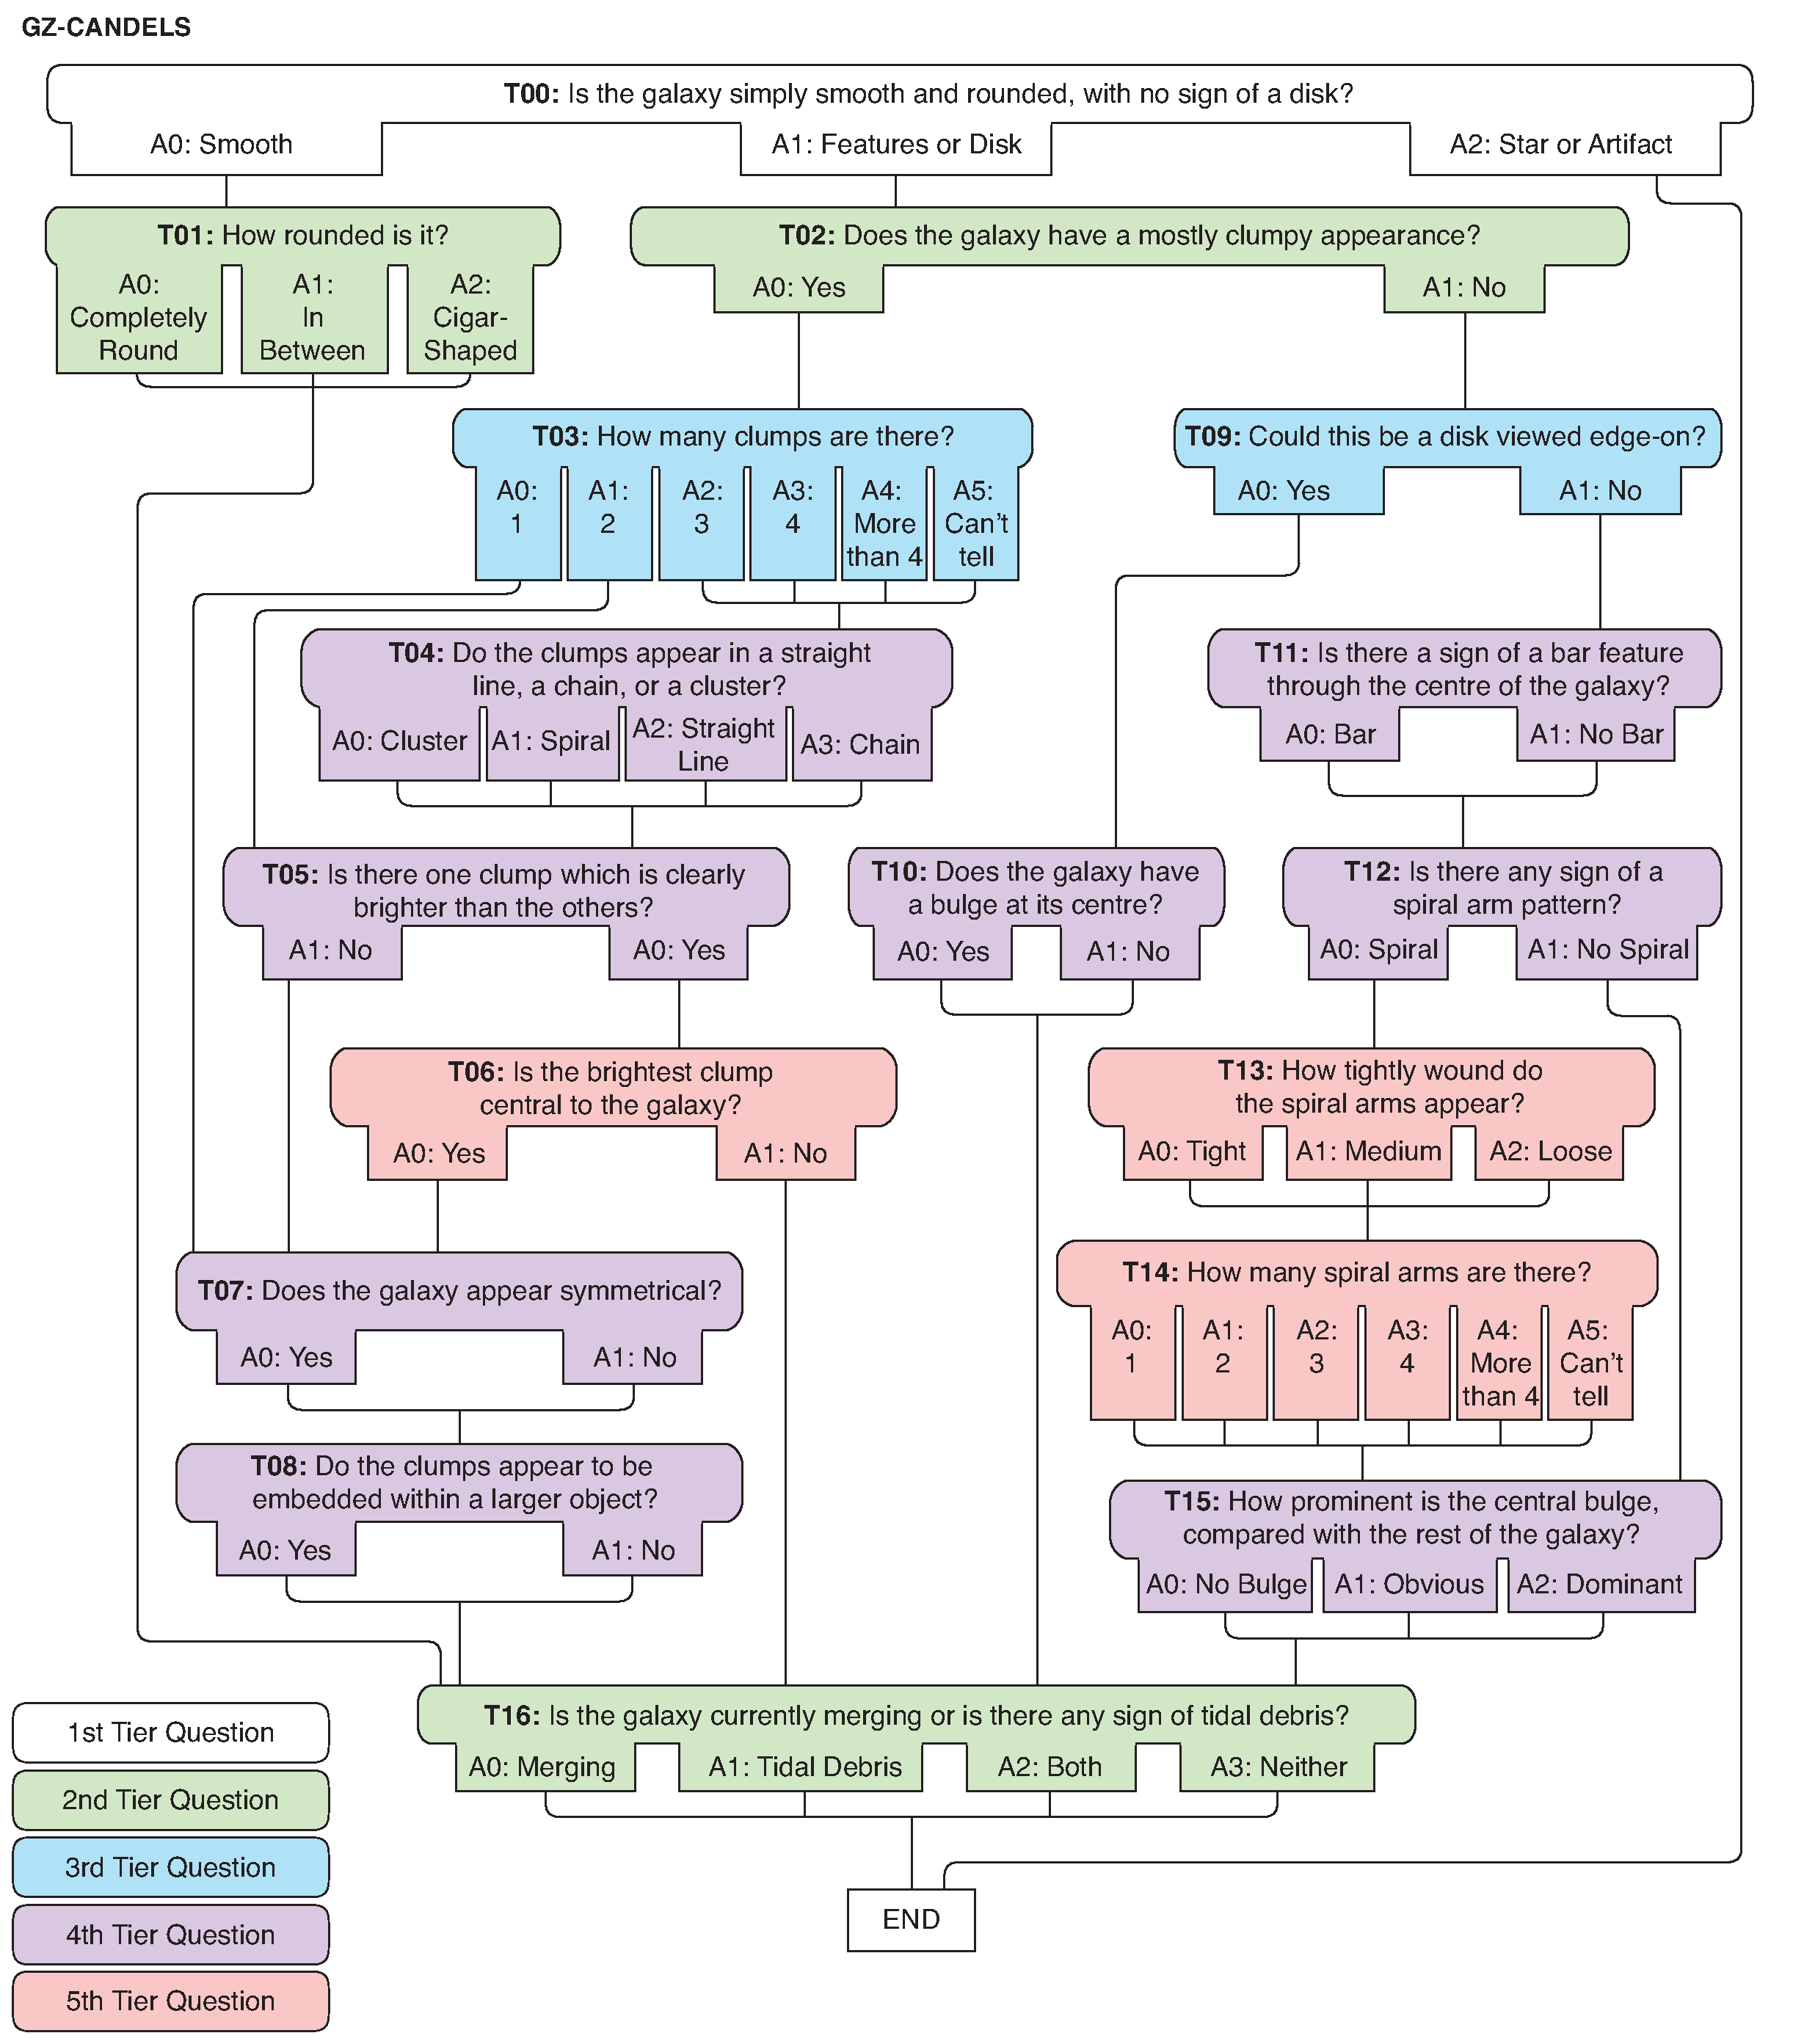
\includegraphics[scale=0.45]{candels_classification_tree_withlabels_new.eps}
\caption{
The Decision Tree for Galaxy Zoo: CANDELS in visual format. There are 16 tasks, with one question per task and up to 6 answers per question. Questions are coloured according to the minimum number of branches prior to that question. All classifiers are asked the first question (task T00), and there are 4 subsequent levels of branching. The tree is also shown in text in Table \ref{table:tree}.
}
\label{fig:tree}
\end{figure*}
%%%%% END FIGURE %%%%%

The goal of Galaxy Zoo CANDELS is to provide detailed quantitative visual morphologies of galaxies observed by the deepest, most complete \emph{HST} multi-wavelength legacy survey to date. 
%The classification interface was designed first and foremost with this goal in mind. 
There are many morphological features of interest, including both broad questions about a galaxy's overall appearance and more detailed questions about specific features. 

We employ a tree-based structure for collecting information on these morphological features, a strategy that has been used successfully in both Galaxy Zoo 2 and Galaxy Zoo: Hubble. The decision tree, shown visually in Figure \ref{fig:tree} and in text in Table \ref{table:tree}, first asks the classifier to choose between the broad categories of ``smooth and rounded'', ``features or disk'', and ``star or artifact''. The next question either exits the classification (if the classifier has indicated the subject is of a star or artifact) or asks for further details about the galaxy. 

If the classifier has indicated in the first question that the galaxy has features or a disk, a series of follow-up questions are asked about features such as clumps, spiral patterns, bulge strength, and the presence of a bar. If the classifier has instead indicated the galaxy is mostly smooth and rounded, the next question asks them to rate the overall roundedness, a question roughly corresponding to an axis ratio measurement. Finally, when the classifier has finished answering all follow-up questions about either the ``smooth'' or ``featured'' galaxy, they are then asked whether the galaxy is undergoing a merger, has tidal tails, or has both, or neither.

The tree-based structure has a number of advantages. First, it collects substantially more information on each galaxy than a single question would, and captures a more detailed classification of higher-order structures while minimising the effort required on the part of the classifier by only asking for relevant inputs based on the answers provided to previous questions. 

Second, it focuses the classifier on a single feature at a time, highlighting each feature. This resets the attention of the classifier with each new question and avoids the problems that may result when a person is presented with a large number of decision tasks at once, including a decrease in optimal decision-making \citep{iyengar00,crescenzi13, besedes15} and a reduced ability to recognise the unexpected \citep{simons99,todd05}. 

Third, the tree-based structure is especially optimal for an interface which may collect classifications from classifiers who have never before seen an image of a galaxy and may seek additional training. Within the interface, the classifier may optionally display training images in a ``Help'' section that shows different examples of the feature relevant to the current question. Asking single-topic questions in turn permits a full set of training images to be available throughout the classification without placing an unnecessary cognitive load on the classifier.

%{\notebsm Other advantages we should mention?}

The disadvantage of a tree-based classification structure concerns the dependencies introduced into the vote fractions by such a structure. A classifier cannot, for example, answer that the same galaxy has both a mostly smooth appearance and also has a spiral feature. This is in some ways an advantage, as it prevents contradictory and unphysical classifications, but it also means that an analysis of  morphological vote fractions with the goal of examining spiral galaxies must account for the fact that whether a given classifier reached the spiral branch of the decision tree depends on their answer to the questions preceding it. 

Accounting for dependencies of questions in deeper branches of the decision tree on higher-level questions is, however, a manageable task which has been undertaken successfully in many previous studies of specific galaxy structural features \citep[for specific examples, see e.g.][]{masters11a,melvin14,galloway15}. We provide guidelines for optimal morphological selection of samples using Galaxy Zoo consensus classifications in Section \ref{sec:usage}.

The Galaxy Zoo CANDELS decision tree is shown in visual form in Figure \ref{fig:tree} and in text form in Table \ref{table:tree}. We note that this tree is most similar to the tree used in the Galaxy Zoo: Hubble project \citep[described in][]{melvin14}, which also has an additional branch identifying clumpy galaxies and focusing on the detailed structure of galaxy clumps. There are small differences, however: for example, Task 10, the question about a bulge in an edge-on disk, is a Yes/No question here, whereas in previous iterations of the decision tree this question also asked whether the bulge shape was rounded or boxy. Additionally, the final question in the tree (Task 16) is substantially different from previous versions and is here only concerned with galaxy mergers and tidal features. 

After the classification of each subject is finished, the classifier is asked ``Would you like to discuss this object?'' If the classifier selects ``No'', a new subject is shown for classification. If the classifier selects ``Yes'', a new window opens with a discussion page focused on the subject they have just classified. Within this part of the Galaxy Zoo software, called Talk, people may ask questions and make comments on specific subjects, or engage in more general discussions. People may also ``tag'' subjects and discussions using a format similar to Twitter's hashtag system. Some of these tags were used in the pre-analysis of Galaxy Zoo CANDELS data, on which more details are given in Section \ref{sec:rawclass} below.



\begin{table*}
 \begin{tabular}{@{}cllr|cllr}
 \hline
\multicolumn{1}{l}{Task} &
\multicolumn{1}{c}{Question} &
\multicolumn{1}{c}{Responses} &
\multicolumn{1}{c}{Next} &
\multicolumn{1}{l|}{Task} &
\multicolumn{1}{c}{Question} &
\multicolumn{1}{c}{Responses} &
\multicolumn{1}{c}{Next} 
\\ 
\hline
\hline						
T00  & {\it Is the galaxy simply smooth       } & smooth            & 01         &  T09  & {\it Could this be a disk viewed   }  & yes              & 10 \\
     & {\it and rounded, with no sign of      } & features or disk  & 02         &       & {\it edge-on?                      }  & no               & 11 \\
     & {\it a disk?                           } & star or artifact  & {\bf end}  &       &                                       &                  &    \\
     &                                          &                   &            &  T10  & {\it Does the galaxy have a        }  & yes              & 16 \\
T01  & {\it How rounded is it?                } & completely round  & 16         &       & {\it bulge at its centre?          }  & no               & 16 \\
     & {\it                                   } & in between        & 16         &       &                                       &                  &    \\
     & {\it                                   } & cigar-shaped      & 16         &  T11  & {\it Is there a sign of a bar      }  & bar              & 12 \\
     &                                          &                   &            &       & {\it feature through the centre    }  & no bar           & 12 \\
T02  & {\it Does the galaxy have a            } & yes               & 03         &       & {\it of the galaxy?                }  &                  &    \\
     & {\it mostly clumpy appearance?         } & no                & 09         &       &                                       &                  &    \\
     &                                          &                   &            &  T12  & {\it Is there any sign of a        }  & spiral           & 13 \\
T03  & {\it How many clumps                   } & 1                 & 07         &       & {\it spiral arm pattern?           }  & no spiral        & 15 \\
     & {\it are there?                        } & 2                 & 05         &       &                                       &                  &    \\
     & {\it                                   } & 3                 & 04         &  T13  & {\it How tightly wound do the      }  & tight            & 14 \\
     & {\it                                   } & 4                 & 04         &       & {\it spiral arms appear?           }  & medium           & 14 \\
     & {\it                                   } & more than four    & 04         &       & {\it                               }  & loose            & 14 \\
     & {\it                                   } & can't tell        & 04         &       &                                       &                  &    \\
     &                                          &                   &            &  T14  & {\it How many spiral arms          }  & 1                & 15 \\
T04  & {\it Do the clumps appear in           } & cluster           & 05         &       & {\it are there?                    }  & 2                & 15 \\
     & {\it a straight line, a chain          } & spiral            & 05         &       & {\it                               }  & 3                & 15 \\
     & {\it or a cluster?                     } & straight line     & 05         &       & {\it                               }  & 4                & 15 \\
     & {\it                                   } & chain             & 05         &       & {\it                               }  & more than four   & 15 \\
     &                                          &                   &            &       & {\it                               }  & can't tell       & 15 \\
T05  & {\it Is there one clump which is       } & yes               & 06         &       &                                       &                  &    \\
     & {\it clearly brighter than the others? } & no                & 07         &  T15  & {\it How prominent is the          }  & no bulge         & 16 \\
     &                                          &                   &            &       & {\it central bulge, compared       }  & just noticeable  & 16 \\
T06  & {\it Is the brightest clump            } & yes               & 07         &       & {\it with the rest of the galaxy?  }  & obvious          & 16 \\
     & {\it central to the galaxy?            } & no                & 16         &       & {\it                               }  & dominant         & 16 \\
     &                                          &                   &            &       &                                       &                  &    \\ 
T07  & {\it Does the galaxy                   } & yes               & 08         &  T16  & {\it Is the galaxy currently       }  & merging          & {\bf end}  \\
     & {\it appear symmetrical?               } & no                & 08         &       & {\it merging or is there any       }  & tidal debris     & {\bf end}  \\
     &                                          &                   &            &       & {\it sign of tidal debris?         }  & both             & {\bf end}  \\
T08  & {\it Do the clumps appear to be        } & yes               & 16         &       & {\it                               }  & neither          & {\bf end}  \\
     & {\it embedded within a larger object?  } & no                & 16         &       &                                       &                  &    \\
 \end{tabular}
 \caption{The Galaxy Zoo CANDELS decision tree, comprising 16 tasks and 51 responses. Each task is comprised of a single question and up to 6 possible responses. The first question is Task 00, and a classification is completed by responding to all subsequent questions until the end of the tree is reached. The `Next' column indicates the subsequent task the classifier is directed to upon choosing a specific response. Although a classifier will flow through the tree from top to bottom, there is no path through the tree that includes all tasks. 
%The texts in `Question' and `Responses' are displayed to classifiers during classification, along with the icons in Figure~\ref{fig-flowchart}.
\label{table:tree}}
\end{table*}



\subsection{Raw classifications}\label{sec:rawclass}

% First classification 2012-09-10 18:41:25 UTC, last classification 2013-11-30 12:58:51 UTC
% NOTE I've just discovered that people who put commas in their usernames can mess up my (admittedly simple and awk-based) system of separating classifications. 
% So I am 99% sure the total number of classifications is 2,149,206 but I'm not 100% sure yet.

%%%%% [FIGURE: Example images] %%%%%
\begin{figure*}
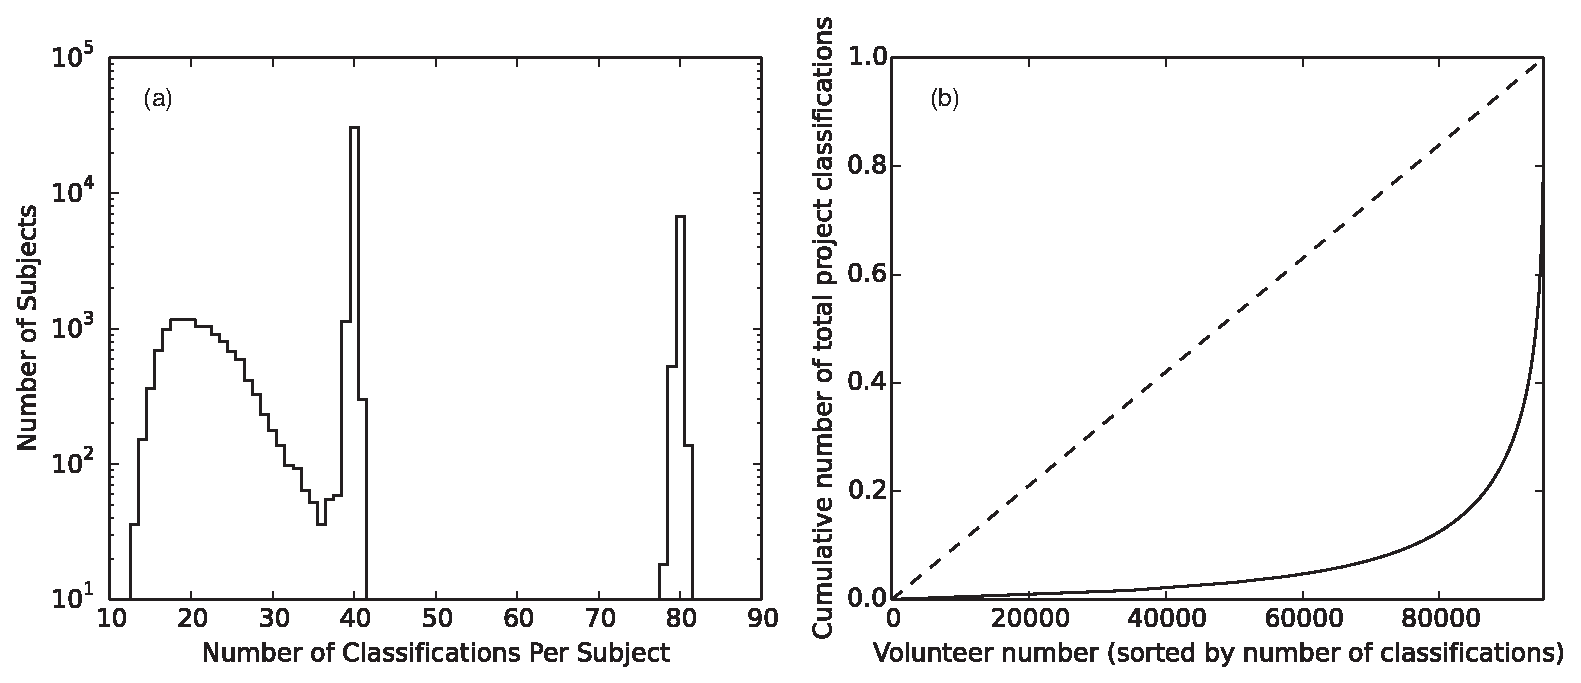
\includegraphics[scale=0.67]{classifications_users_basicinfo.eps}
\caption{
Basic information on classifications. \emph{Left}: Distribution of (unweighted) number of classifications per subject in Galaxy Zoo CANDELS. The majority of subjects have 40 independent classifications each; a subset of 13,392 were retired early after being identified as too faint and low-surface-brightness for additional classifications to be useful (11,837) or as stars or artifacts (1,555). Subsequently, 7,402 subjects where at least 20\% of classifiers registered a vote for ``Features or Disk'' in the first task were re-activated with a retirement limit of 80 classifications, in order to ensure a complete sampling of the deepest branches of the question tree. \emph{Right}: Cumulative distribution of classifications per classifier, where the classifiers are sorted in order of least to most classifications contributed (Lorenz curve for classifiers). If every classifier had contributed the same number of classifications, the Lorenz curve would be equal to the dashed curve. The top 9\% of classifiers contributed 80\% of the classifications (Gini coefficient = 0.86). 
}
\label{fig:classification_basic_info}
\end{figure*}
%%%%% END FIGURE %%%%%


The first classification of a subject from CANDELS was registered on the Galaxy Zoo interface\footnote{zoo4.galaxyzoo.org} on the 10th of September 2012. The final classification considered here, in the first phase of Galaxy Zoo CANDELS, was registered on the 30th of November 2013. Between these times, the site collected 2,149,206 classifications of 52,073 CANDELS subjects (of which 2,518 were intentional duplicates of the same galaxy; see Section \ref{sec:depth}) from 41,552 registered classifiers and 53,714 web browser sessions where the classifier did not log in. For all analysis presented here we have assumed that each unregistered browser session contains classifications from a single, unique classifier. 

Subjects within a given Galaxy Zoo sample are chosen randomly for classification, so that the number of independent classifications per galaxy builds up uniformly through the full sample. Once a pre-set classification limit has been reached, the subject is retired from the active classification pool. The initial goal for Galaxy Zoo CANDELS was to obtain at least 40 independent classifications for each galaxy. 

This uniform retirement limit was modified twice during the project. In the first instance, a pre-analysis of the dataset performed when the average number of classifications per galaxy had reached approximately 20 revealed 11,837 subjects where further classification was unlikely to provide significant additional information. These subjects were identified with the help of a set of subjects tagged in the Galaxy Zoo Talk software as ``\#toofainttoclassify'' and ``\#FHB'' (which stands for ``Faint Hubble Blob''). Tags in Galaxy Zoo Talk are generally highly incomplete; thus the 204 tagged subjects were used as tracers during a further examination of all subjects in magnitude-surface brightness parameter space. The selection, made from initial photometry, was deliberately conservative, retiring only those subjects where it was clear that the classification vote fractions had converged at all tiers of the classification tree. During this analysis, an additional 1,555 subjects were identified as highly likely to be stars or artifacts and were also retired.

The second modification of the retirement limit was implemented 1 year after the project start. At this time, the retirement limit was raised to 80 classifications for all galaxies where at least 20\% of classifiers had answered ``Features or Disk'' to the first question (task T00 in Figure \ref{fig:tree} and Table \ref{table:tree}). This is a higher retirement limit than in previous Galaxy Zoo projects, and it is justified by the increased complexity of the question tree compared to, e.g., Galaxy Zoo 2 \citep{willett13}. The Galaxy Zoo CANDELS question tree has an additional branch level, and the number of classifiers answering a question is typically reduced at each branch point. Thus, 40 classifications at the first question may not be enough to ensure convergence in, for example, task 14, ``How many spiral arms are there?'', a 5th-tier question with 6 possible answers. The increased retirement limit affected 7,402 subjects.

Figure \ref{fig:classification_basic_info}a shows the distribution of total classification counts within the sample. The majority of subjects received 40 classifications, but the distribution is asymmetric: there are peaks at $\sim 20$, $40$, and $80$ classifications, consistent with the description above. The Lorenz curve of classifications is shown in Figure \ref{fig:classification_basic_info}b. The curve is highly skewed from the $1:1$ line that would be seen if all classifiers contributed the same number of classifications; the top 9\% of classifiers contributed 80\% of total classifications. The Gini coefficient for classfications, i.e., the fractional difference in area under the Lorenz curve versus the dashed line, is 0.86. This is typical of past Galaxy Zoo projects and Zooniverse citizen research projects in general \citep{cox15}. 

The values in Figure \ref{fig:classification_basic_info} are raw classification counts; while raw classification counts and vote fractions are certainly useful, we additionally ``clean'' the data with a simple method to identify seriously errant classifiers (most likely from bots), and then apply a classifier weighting scheme to classifications to produce a cleaner set of vote fractions for each subject. Both steps are described in further detail below.

\subsection{Identification and removal of single-answer prolific classifiers}\label{sec:bots}

Only a small number of unresolved sources or sources dominated by an unresolved element (i.e., stars and quasars) are included in the full Galaxy Zoo CANDELS subject sample. Examination of the CANDELS photometric catalogs \citep[][M. Peth et al., in preparation]{galametz13,guo13} shows that less than 12 per cent of subjects have $\stellarity > 0.25$ (a very inclusive cut; a more typical cut on stellarity estimates the number of unresolved sources at less than 3 per cent). If the subjects assigned to a classifier are drawn at random from the subject set, then for any classifier who submits a substantial number of classifications, the chances they will be shown a large fraction of stars is very small. 

Even for more common answers to the first task, the chances of a classifier being randomly assigned a highly uniform set of $N$ subjects becomes very small as $N$ becomes large. For example, if the probability of being assigned a ``smooth'' galaxy is $p = 0.9$, the chance of being assigned a subject set of 98 per cent smooth galaxies out of $N > 200$ total is so small that it would likely happen approximately once per billion classifiers, \emph{i.e.}, it is highly unlikely in a project with $\sim 100,000$ classifiers.

% "small group" below = 86 classifiers
Within the raw classifications, a small group of classifiers (86, or less than 0.1 per cent) classified at least 200 subjects \emph{and} gave the same answer to the first question at least 98 per cent of the time. Within this group, 99.6 per cent of classifications were for ``star or artifact'' (from 84 classifiers) and 0.4 per cent were for ``smooth'' (from 2 classifiers). As the chances of any classifier being actually served $> 98$ per cent of subjects with the same intrinsic classification in more than 200 classifications is vanishingly small, these classifiers are most likely bots or are otherwise not actually engaging in the classification task. While these classifications ($6.8$ per cent of the total classifications) would be substantially down-weighted during the classifier weighting process described below, we formally omit them from further analysis and do not include them in the weighting and consensus calculations. 

\subsection{Classifier Weighting} \label{sec:weighting}

Multiple methods of classifier weighting have been successfully employed by many different Zooniverse projects \citep{lintott08, bamford09, lintott11, esimpson12, rsimpson12, schwamb12, johnson15, marshall16}. In general, the optimal choice of classifier weighting depends on the amount of information available per subject and the goal of the project. In Galaxy Zoo CANDELS the goal is to converge to a classification for each galaxy whilst still allowing for unexpected discoveries, and there is ample information from classifiers but little information on the ``ground truth'', i.e., we do not know what the true intrinsic classification is for even a modest fraction of the sample.

For these reasons, we apply a consensus-based weighting method for the majority of the tasks in the decision tree, informed first by the application of initial weights based on comparison of the classifications in the first question to the stellarity (\stellarity ) parameter from the CANDELS photometric catalogs. Both are described below, in the order in which they are applied.

\subsubsection{Initial weighting based on ``Star'' versus ``Galaxy'' classifications}

In the initial classification task (T00), we ask classifiers to separate stars from galaxies and identify a galaxy as ``smooth'' or ``featured''. Although we have no ``ground truth'' information on the overall morphology of a galaxy, we do have very reliable information on whether the source detected in each image is extended, from the \stellarity\ parameter. We can therefore apply classifier weightings to this task based on whether classifiers typically classify bright stars as ``star or artifact'', and whether they classify extended objects as galaxies (i.e., whether they answer \emph{either} ``smooth'' or ``featured'').

We select a sample of bright stars having $F160W < 18.5$ and $\stellarity  > 0.8$ from within the Galaxy Zoo-CANDELS subject set. After manually rejecting 2 subjects which contain a galaxy in the central image position with a bright star nearby or overlapping, the bright-star gold-standard sample contains 263 subjects.

We select a sample of extended sources having $F160W < 25$ and $\stellarity < 0.03$, with further manual removal of images with artifacts and other ``unclassifiable'' sources. We first cleaned this sample by rejecting remaining sources where more than 65 per cent of classifiers had selected the ``star or artifact'' response to task T00, a choice made to favour purity of the extended-source sample over completeness. We additionally rejected 398 artifacts falling below this threshold, leaving a total of 29,996 subjects in the extended-source gold-standard sample. 

Having selected these samples, we then assigned an index $n_s$ to each subject classification from within either gold-standard subject set. For subjects within the bright-star gold-standard set, the classification index was set to $n_s = -1$ if the classifier had \emph{not} marked the subject as ``star or artifact'', and was $n_s = 0$ otherwise. For subjects within the extended-source gold-standard set, the classification index was set to $n_s = -1$ if the classifier had marked the subject as ``star or artifact'', and was set to $n_s = +1$ otherwise.

We then define the index $n_c$ for each classifier as the sum of all their classification indices $n_s$, and the weight for task T00 is assigned based on the classifier index as
\begin{equation}
   w_{00}= \left\{
    \begin{array}{l l}
      \max \left(1.1^{n_c}, 0.01\right)       & \text{ if } n_c < 0 \\
      \min \left(1.05^{n_c}, 3 \right) & \text{ if } n_c \geq 0.\\
    \end{array} \right.
    \label{eqn-seedweight}
 \end{equation}

This weighting results in a set of classifier weights between $0.01 < w_{00} < 3$, with classifiers whose classifications are generally ``correct'' being up-weighted and classifiers who are more often ``incorrect'' being down-weighted.  79 per cent of classifiers classified at least 1 subject within either gold-standard subject set; classifiers who did not classify any subjects in the gold-standard subject set have $w_{00} = 1$. Of the classifiers who were included in the weighting, 56 per cent have $w_{00} > 1$, with a mean of $\left< w_{00} \right> = 1.11$. As a last step, the weights are re-normalised so that the sum of weights is equal to the total number of classifications.

Following this initial weighting, we create an initial set of vote fractions for each subject by summing the weighted votes for each task and response, and reporting the vote fractions $f$ for each. We use this as an initial consensus classification catalog in the consensus-based weighting applied to the remaining tasks, described in further detail below.

\subsubsection{Consensus-based classifier weighting}

Following the weighting of task T00 described above, we adopt an iterative consensus-based weighting method for classification tasks T01 through T16. This weighting scheme follows previous Galaxy Zoo projects and effectively identifies the small proportion of classifiers whose contributions are routinely errant compared to other classfiers (or consistent with random inputs) and downweights their contributions, while preserving the inputs from the vast majority of classifiers.

Weights for each classifier are computed based on a mean consistency factor, \kappamean , which is the average of consistencies for each of that classifier's classifications. For a given classification $i$ composed of a series of completed tasks $t$ answered about a specific subject, we compare the classifier's answer to each task with the aggregated classifications of all classifiers of the same subject. Each task has $a_t$ answers from all classifiers, each of which is assigned to one of $N_{r,t}$ possible responses to the task. We define the vote fraction for a particular response $r$ as $f_r \equiv a_r/a_t$, where $a_r$ is the number of positive answers for that response (i.e., the number of classifiers who selected that response out of all possible responses to the task).

For each task that was completed by the classifier in classification $i$, the consistency index $\kappa_r$ for each response $r$ to that task $t$ is 
\begin{equation}
    \kappa_r = \left\{
    \begin{array}{l l}
      f_r       & \text{ if the classifier's answer corresponds} \\
                  & \text{ to this response,}\\
      (1 - f_r) & \text{ if the answer does not correspond.}\\
    \end{array} \right.
    \label{eqn-consistency-r}
 \end{equation}
The consistency for that task, $\kappa_t$, is the average of these indices over all possible responses. For example, if a classifier responded ``Star or Artifact'' to Task T00 for a particular subject, and the overall vote fractions on that task for that subject are $($``Smooth'', ``Features or Disk'', ``Star or Artifact''$) = (0.1, 0.6, 0.3)$, then the classifier's consistency for Task T00 for this classification is
$$
\kappa_t = \left[\left(1 - 0.1\right) + \left(1 - 0.6\right) + 0.3\right]/3 = 0.5\overline{3}.
$$
In the above example, the classifier's answer to Task T00 leads to the end of the workflow (Table \ref{table:tree}), so this $\kappa_t$ is also equal to the classifier's consistency for the overall classification, $\kappa_i$. More generally, the classification consistency is the answer-weighted average of the task consistencies:
\begin{equation}
\kappa_i = \frac{\sum_t \kappa_t a_t}{\sum_t a_t} ,
\label{eqn-consistency-i}
\end{equation}
where each sum is over the number of tasks the classifier completed during the classification.

Following this calculation for the entire classification database, each classifier's average consistency is calculated as
\begin{equation}
\mkappamean = \frac{1}{N_i} \sum_i \kappa_i .
\label{eqn-consistency-avg}
\end{equation}

Averaging over a classifier's individual consistency values for all classifications effectively downweights those contributions from classifiers whose classifications regularly diverge from the consensus whilst preserving the diversity of classifications from classifiers who are \emph{on average} consistent with each other. It also allows for the classifications of skilled classifiers to remain highly weighted even on difficult subjects where the individual consensus is skewed (e.g., if an image is very noisy or if a nearby artifact is distracting to less experienced classifiers). 

The classifier weight is then calculated as 
\begin{equation}
w = \min \left(1.0,(\mkappamean / 0.6)^{8.5} \right) ,
\label{eqn-weight}
\end{equation}
a formulation that preserves a uniform weighting for any classifier with $\mkappamean \geq 0.6$ and downweights those with a lower consistency rating.

The weighted consensus classifications are then calculated for each subject by summing the weighted votes for each task and response between task T01 and T16, and reporting the vote fractions $f$ for each. (Although the classifications for task T00 are included in the computation of the consensus-based weights, the vote fractions for task T00 are not re-computed using the consensus-based weights.) As the classifier weights are calculated via comparison with the consensus, which leads to a new consensus, this method can be iterated until the classifier weights converge to a stable value. 

In practice, the number of iterations required to reach this goal is low \citep[e.g., 3 or less in previous projects;][]{bamford09,willett13}. In Figure \ref{fig:consistencies} we show the distribution of classifier consistencies after 1-5 iterations of the above method. Between the 4th and 5th iterations, 99 per cent of consistency values varied by less than 0.6 per cent. After 5 iterations, approximately 3 per cent of classifiers have consistency $\mkappamean < 0.5$ (corresponding to a weight $w \lesssim 0.2$), whereas 85 per cent of classifiers have an end weight of $w = 1$. The vast majority of Galaxy Zoo classifiers contribute highly valuable information to the project.

Figure \ref{fig:exampleclass} shows examples of galaxies with different weighted consensus classifications for several of the tasks described in Table \ref{table:tree} and Figure \ref{fig:tree}. 

%%%%% [FIGURE: classifier Consistencies] %%%%%
\begin{figure}
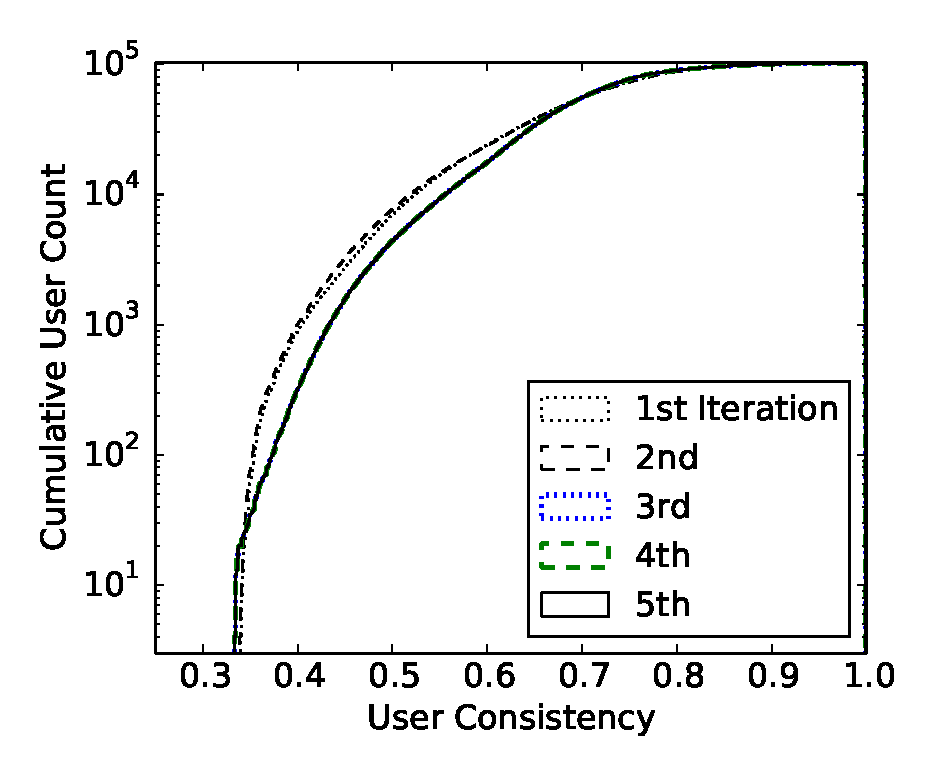
\includegraphics[scale=0.57]{consistencies_iterations2.eps}
\caption{
Distribution of classifier consistencies \kappamean\ after 1 (black dashed), 2 (black dotted), 3 (thick blue dotted), 4 (thick green dashed), and 5 (black solid) iterations of the consistency-based weighting method  (described in Section \ref{sec:weighting}). Convergence of this method requires relatively few iterations: further iterations do not change significantly from the solid curve. Approximately 85 per cent of classifiers have $\mkappamean \geq 0.6$ and weights $w = 1$. 
}
\label{fig:consistencies}
\end{figure}
%%%%% END FIGURE %%%%%


%%%%% [FIGURE: Example images] %%%%%
\begin{figure*}
\includegraphics[scale=1.45]{mosaic_sm.eps}
\caption{
Example (inverted) galaxy images for different consensus classifications of different responses to tasks in the Galaxy Zoo CANDELS classification tree. From top to bottom row, the responses are: Task 00, ``Smooth''; Task 00, ``Featured''; Task 00, ``Star or Artifact''; Task T02, ``Yes'' (Clumpy); Task T09, ``Yes'' (Edge-on); Task T12, ``Yes'' (Spiral); Task T16, ``Merging''. Each image is labelled with the weighted percentage of total votes for that task that were registered for that response, with the weighted vote percentage increasing from left to right. The galaxies were selected after following the suggestions in Section \ref{sec:usage} regarding selection of appropriate samples, including restrictions on votes from earlier branches in the tree (see Figure \ref{fig:tree} for more information on branches).
}
\label{fig:exampleclass}
\end{figure*}
%%%%% END FIGURE %%%%%


% Postponing this as the IBCC classifications are a little weird - we need a bigger training set.
%\subsubsection{IBCC}



%\subsection{Surface Brightness and Classification Bias}\label{sec:biases}

%The consistency-based weighting described above ensures the preservation of the way in which the variety of classifications echoes the confidence level in any individual response, while ensuring expert classifiers remain highly weighted and the very small fraction of errant classifiers are down-weighted.

%However, the amount of information available per subject varies: the CANDELS survey takes images at multiple depths, and the galaxies themselves have a wide range of intrinsic brightnesses and distances. Even at a given redshift, the classification of a galaxy depends on both its luminosity and size (i.e., its surface brightness). In particular, as the observed surface brightness of a galaxy decreases it tends to appear more smooth compared to the image noise, decreasing the detection of features \citep{bamford09,willett13}.

%Previous Galaxy Zoo projects examining galaxies in the more local Universe have accounted for this bias by using less distant galaxies to determine how to debias the classifications of more distant galaxies as a function of redshift. This is effective under the assumption that the underlying distribution of classifications is invariant with redshift. This is clearly an inappropriate assumption in the case of a deep \emph{HST} survey such as CANDELS, where 80 per cent of subjects fall within the redshift range $0.25 < z < 3.5$, over which galaxy shapes most certainly evolve.

%Despite these challenges, Galaxy Zoo classifiers have proven extremely reliable at classifying features which are visible above some surface brightness detection limit. When the overall surface brightness of a galaxy falls below that limit, the detection of locally more bright features may still be achieved, but in general the classification vote fraction of a galaxy as ``featured'' may be considered a lower limit. We describe below the effect of surface brightness limit on Galaxy Zoo CANDELS classifications and discuss the implications for usage of the vote fractions.


%\subsubsection{Surface brightness limits in Galaxy Zoo CANDELS}\label{sec:sb}

%We aim to determine empirically the surface brightness threshold above which Galaxy Zoo CANDELS classifications reliably characterise the level of ``features'' present in a galaxy. It is therefore important to choose a subset of galaxies so as to minimise the dependence of a galaxy's ``true'' classification on factors such as distance and luminosity.

%We define the observed surface brightness of a galaxy using the magnitude and size reported in the CANDELS photometric catalogs for each field \citep[][Peth et al., in preparation]{guo13,fill_in,later}. Specifically, we use the $F160W$ \textsc{auto} fluxes and the radius containing 80\% of the galaxy light, $r_{80}$, to determine a representative surface brightness for each galaxy. We also use the measured axis ratios $b/a$, dividing the flux by the area contained within an ellipse of area $\pi a_{80} b_{80}$, in square arcseconds. We then convert to magnitudes, resulting in a single surface brightness $\mu_{\textsc{auto}}$ in mag/arcsec$^2$ for each subject. 

%We then choose a subset of subjects from the full sample described above within a narrow range of redshifts to minimise evolutionary effects. We use galaxies with $1.1 < z < 1.4$, spanning an evolutionary period of $\sim 1$~Gyr, but note the analysis is insensitive to the specific choice of redshifts so long as the bin spans a similar time period.

%Figure \ref{fig:sb_z1} shows the vote fractions for the response ``Features or Disk'' in the first question (task T00) in the decision tree, versus surface brightness. The variation in the distribution of featured classifications with surface brightness is apparent even after disregarding subjects with $\mu_{\textsc{auto}} < 20$~mag/arcsec$^2$, which are typically stars. The right panel of Figure \ref{fig:sb_z1} shows these distributions as cumulative histograms binned by $\Delta \mu_{\textsc{auto}}$. As expected, the distribution of featured vote fractions changes with surface brightness, with all vote fraction distributions being similarly lacking in detected features for observed $\mu_{\textsc{auto}} > 23.0$~mag/arcsec$^2$.  

%Therefore, although we report vote fractions for all subjects in the Galaxy Zoo CANDELS catalog, including those with $\mu_{\textsc{auto}} > 23$, we strongly urge caution when using classifications of galaxies fainter than this surface brightness level. Featured vote fractions at surface brightnesses fainter than this may be reasonably considered lower limits, as many features may not be visually apparent. In all subsequent analysis in this paper, we consider only galaxies with $\mu_{\textsc{auto}} < 23.0$ unless otherwise specified. 


%%%%% [FIGURE: Surface Brightnesses] %%%%%
%\begin{figure*}
%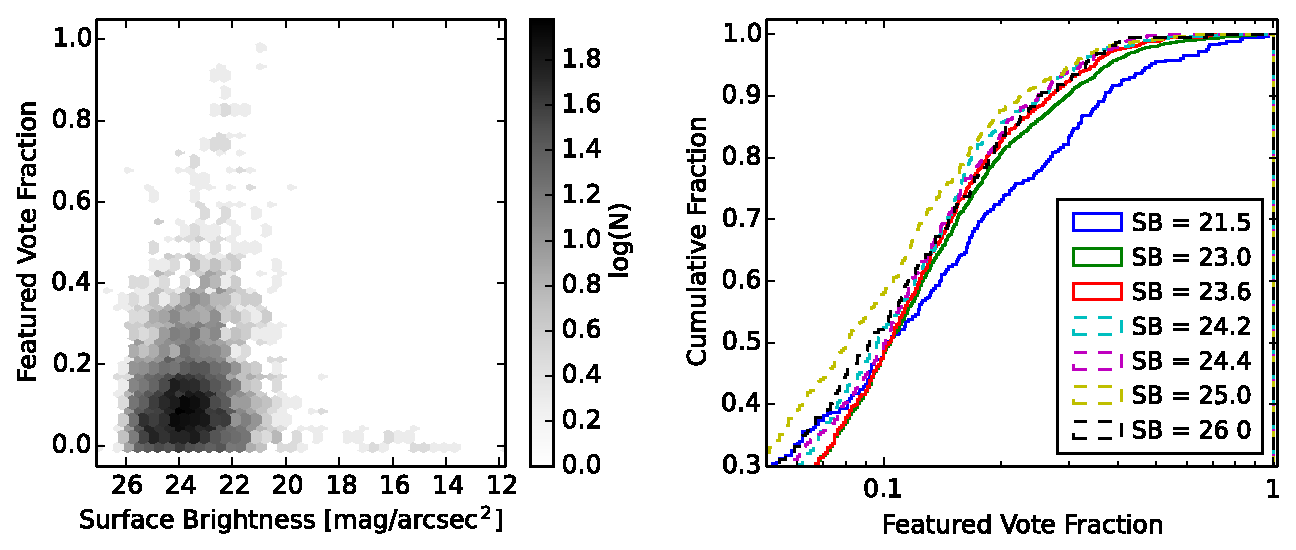
\includegraphics[scale=0.8]{sb_z1.eps}
%\caption{
%Comparison of subject surface brightnesses and vote fractions for the response ``Features or Disk'' in the first task (T00) of Galaxy Zoo CANDELS for subjects with $1.1 < z < 1.4$. \emph{Left:} 2-D histogram of $f_{\rm features}$ versus $\mu_{\textsc{auto}}$, with shading of each hexagonal bin indicating the number of subjects in that bin. Subjects with  $\mu_{\textsc{auto}} < 20$~mag/arcsec$^2$ are generally point-like sources. The distribution of featured vote fraction is a function of surface brightness. \emph{Right:} Cumulative distributions of $f_{\rm features}$ in bins of surface brightness. Although we note that some of the variations seen are likely due to intrinsic differences in populations at different luminosities, there is a clear and strong change in the distribution at $\mu_{\textsc{auto}} \approx 23.0$. 
%}
%\label{fig:sb_z1}
%\end{figure*}
%%%%% END FIGURE %%%%%



%\subsubsection{The effect of image depth on classifications}

%Old words
%80 per cent of all subjects in Galaxy Zoo CANDELS have redshifts $0.25 < z < 3.5$, over which cosmological distances galaxies of identical luminosities will have observed fluxes that differ by orders of magnitude. The angular diameter distance, meanwhile, varies in a very different way (and indeed does not evolve much beyond $z \sim 1$ compared to the luminosity distance). 


\subsection{Use of Classifications in Practice}\label{sec:usage}

The branched nature of the decision tree (Figure \ref{fig:tree}) means that selection of a sample of galaxies for a given morphological investigation may depend on a number of factors. For example, it is possible to choose a quantitative threshold for selection of a sample of galaxies with a given feature or combination of features corresponding to one's optimal trade-off between sample completeness and purity. One may also weight a population analysis by the vote fraction for a particular morphological feature \citep[making the assumption that the probability of a galaxy having that feature, or the strength of the feature, is a function of the vote fraction, e.g.,][]{smethurst15}. However, for all tasks below T00 in the tree, it is important to consider the responses to the tasks above that question in this analysis.

For example, a study with the goal of examining spiral galaxies would ideally use a sample selected by considering the responses to task T12, ``Is there any sign of a spiral arm pattern?'' If a pure sample of galaxies with clear spiral arms is desired, a threshold may be selected at a high vote fraction for $f_{\rm spiral}$. If the threshold considers only this vote fraction, however, the final sample will likely be contaminated by galaxies where the spiral vote fraction is dominated by noise because only a small number of people reached that task (e.g., a warped edge-on disk). 

In order to reach task T12, a classifier must give specific answers to the questions ``Is the galaxy simply smooth and rounded, with no sign of a disk?'' (T00), ``Does the galaxy have a mostly clumpy appearance?'' (T02), and ``Could this be a disk viewed edge-on?'' (T09). Each of these classifications should be considered in the context of this hypothetical study's goals in order to select as pure a sample as possible whilst minimising contamination and bias.

If a moderately complete sample is desired, for example, the user could select thresholds for the selection such as $f_{\rm features} > 0.5$, $f_{\rm not\ clumpy} > 0.5$, $f_{\rm not\ edge-on} > 0.5$. Because most galaxies with these classifications will have received 80 classifications apiece (Section \ref{sec:rawclass}), these chained thresholds mean the minimum number of classifiers who will have answered the spiral question for subjects that are included in the sample is $80 \times 0.5^3 = 10$. Higher thresholds will further increase the minimum number of respondents to the deeper-branched question. If lower thresholds are desired, we recommend that the selection explicitly require a minimum number of respondents to each task. 

There is no single set of thresholds that is ideal for all situations. However, in the data release accompanying this paper, we include ``clean'' selections of galaxies with different morphological features. These are detailed further below, but we additionally encourage users of this rich data set to experiment with different threshold/weight combinations in order to achieve their scientific goals.

\subsection{Data release and ``clean'' samples}\label{sec:release}

This paper includes the release of the raw and weighted classifications for each of the $49,555$ subjects in the Galaxy Zoo CANDELS sample. In addition to each raw and weighted vote fraction for each task, we include the raw and weighted number of answers to each task, as well as for the whole galaxy overall. This combines for a total of 136 quantities for each subject, not including the subject ID or any other metadata. This is too much information to present a meaningful sample table in print here. However, the data is structured thusly for each task number $NN$ with $i = {0 {\rm\ to\ } n-1}$ responses:
%oh god it's really late and I just said "thusly"

\begin{itemize}
\item[] \small{\tt t[$NN$]\_[quest\_abbrev]\_a[$i$]\_[resp\_abbrev]\_frac} : the raw fraction of classifiers who gave this response. {\tt quest\_abbrev} and {\tt resp\_abbrev} are abbreviated versions of the specific question and response, respectively.

\item[] \small{\tt t[$NN$]\_[quest\_abbrev]\_a[$i$]\_[resp\_abbrev]\_weighted\_frac} : the weighted fraction of classifiers who gave this response. 

\item[] \small{\tt t[$NN$]\_[quest\_abbrev]\_count} : the raw count of classifiers who responded to this task. 

\item[] \small{\tt t[$NN$]\_[quest\_abbrev]\_weight} : the weighted count of classifiers who responded to this task. 

\end{itemize}

For example, the information available for task T00, which has 3 responses, is structured as:

\begin{itemize}
\item[] \small{\tt t00\_smooth\_or\_featured\_a0\_smooth\_frac}

\item[] \small{\tt t00\_smooth\_or\_featured\_a1\_features\_frac}

\item[] \small{\tt t00\_smooth\_or\_featured\_a2\_star\_or\_artifact\_frac}

\item[] \small{\tt t00\_smooth\_or\_featured\_a0\_smooth\_weighted\_frac}

\item[] \small{\tt t00\_smooth\_or\_featured\_a1\_features\_weighted\_frac}

\item[] \small{\tt t00\_smooth\_or\_featured\_a2\_star\_or\_artifact\_weighted\_frac} 

\item[] \small{\tt t00\_smooth\_or\_featured\_count} 

\item[] \small{\tt t00\_smooth\_or\_featured\_weight}

\end{itemize}

The sum of raw  {\tt \_frac} fractions adds to 1.0, as does the sum of {\tt \_weighted\_frac} fractions. Multiplying the {\tt \_frac} values (raw fractions) by the {\tt \_count} (raw classifier counts) will retrieve the number of people who gave a specific response; likewise with weighted answer counts from {\tt \_weighted\_frac} and {\tt \_weight}. As the consensus-based classifier weighting described in Section \ref{sec:weighting} assigns a weight of $w \leq 1$ to each classifier, the weighted vote count for tasks T01-T16 must be less than or equal to the raw vote count for those tasks. While the raw vote counts and fractions are provided for completeness, we recommend that users of this data set use the weighted fractions and counts.

In addition to the vote fractions for each subject, we provide a set of flags for each subject that indicates its member or non-member status in a ``clean'' sample of galaxies of a specific type. We select separate clean samples of smooth, featured, clumpy, edge-on, and spiral galaxies. These samples contain exemplars of each galaxy type with minimal contamination of the sample, and are correspondingly highly incomplete. They are selected according to the following thresholds using weighted vote fractions:

\begin{itemize}

\item[] \textbf{Smooth} - Task T00: $f_{\rm smooth} > 0.9$, $f_{\rm star\ or\ artifact} < 0.2$

\item[] \textbf{Featured} - Task T00: $f_{\rm features} > 0.9$, $f_{\rm star\ or\ artifact} < 0.2$

\item[] \textbf{Clumpy} - Task T00: $f_{\rm smooth} > 0.9$, $f_{\rm star\ or\ artifact} < 0.2$; Task T02: $f_{\rm clumpy} > 0.8$

\item[] \textbf{Edge-on} - Task T00: $f_{\rm smooth} > 0.9$, $f_{\rm star\ or\ artifact} < 0.2$; Task T02: $f_{\rm not\ clumpy} > 0.5$; Task T09: $f_{\rm edge-on} > 0.7$

\item[] \textbf{Spiral} - Task T00: $f_{\rm smooth} > 0.9$, $f_{\rm star\ or\ artifact} < 0.2$,; Task T02: $f_{\rm not\ clumpy} > 0.5$; Task T09: $f_{\rm not\ edge-on} > 0.7$; Task T12: $f_{\rm spiral} > 0.8$

\end{itemize}


We provide these flags for the convenience of the end user, but we additionally encourage those wishing to use Galaxy Zoo classifications to investigate whether a different set of thresholds would be optimal for their own science case.





\subsection{Depth Corrections}\label{sec:depth}

As outlined in Section \ref{sec:images}, the depth of the CANDELS survey varies substantially between two types of fields, from shallower ``wide'' fields with $\sim 1$ orbit depth in $F160W$ to ``deep'' fields with $\gtrsim 4$ times the overall depth of the wide fields. 

Because different morphological signatures have different characteristic surface brightnesses and light profiles (e.g. clumps, tidal signatures, spheroids, disks), we expect the morphological classifications of subjects to vary somewhat based on the imaging depth. For a survey such as CANDELS that is already relatively deep, we expect this effect to generally be small, but nevertheless using classifications based on imaging from both the wide and deep fields could complicate some scientific inquiries.

To measure and correct for this, shallower images of a sub-sample of ``deep'' subjects were created and added to the active subject sets. These images (from 2,518 subjects in the GOODS-South deep field; hereafter the ``deep-shallow'' subset) are of comparable depth to the wide fields. By comparing the shallower and deeper weighted consensus classifications of these subjects, we determine typical depth corrections to all deep-field subject morphologies, as a function of deep-exposure morphology and galaxy surface brightness.

We define the observed surface brightness of a galaxy using the magnitude and size reported in the CANDELS photometric catalogs for each field. Specifically, we use the $F160W$ \textsc{auto} fluxes and the radius containing 80\% of the galaxy light, $r_{80}$, to determine a representative surface brightness for each galaxy. We also use the measured axis ratios $b/a$, dividing the flux by the area contained within an ellipse of area $\pi a_{80} b_{80}$, in square arcseconds. We then convert to magnitudes, resulting in a single surface brightness $\mu_{\rm{SB}}$ in mag/arcsec$^2$ for each subject.

Figure \ref{fig:depthcorr} shows the difference between shallower and deeper weighted consensus classifications as a function of surface brightness and deep-exposure morphology for two example tasks, T00 and T09. When determining depth corrections for each task, we consider subjects which received more than 10 answers to the question presented by the task, and we also remove 42 bright stars with $\mu_{\rm SB} > 17$ (the mean weighted ``star or artifact'' vote fraction for these is $f_{\rm artifact} = 0.89$). For tasks T01-T16, we additionally remove subjects with $f_{\rm artifact} \geq 0.5$. We then determine a best-fit plane to the change in vote fraction, $\Delta f_r$, for each response as a function of galaxy surface brightness and the vote fraction $f_r$ for the deep-exposure image. If fewer than 75 subjects received at least 10 responses to a particular question, the correction is assumed to be 0 for that question.

The best-fit planes for each response to each task can be used to predict the wide-field depth classifications for each galaxy in the deep fields, in this paper and in future releases of Galaxy Zoo-CANDELS data.  For the 8,130 subjects with $F160W$ limiting magnitudes at least as faint as the brightest limiting magnitude in the deep-shallow subset but for which we do not also have separate wide-field depth classifications, we use their vote fractions for each task and response, $f_r$, and their surface brightnesses $\mu_{\rm SB}$, to interpolate corrections $\Delta f_r$ along the best-fit plane for each task and response. Where a $\left( f_r, \mu_{\rm SB} \right)$ pair is outside the area defined by the data (blue points in Figure \ref{fig:depthcorr}), we assume the correction is equal to the value of the correction at the nearest boundary defined by the projection of the data in the deep-shallow subset onto the best-fit plane (that is, we do not extrapolate). 

In addition to the release of classification data described in Section \ref{sec:release} above, we additionally present these ``corrected'', weighted classifications for each of the 8,130 subjects with deep exposures but for which we do not also have separate wide-field depth classifications, as well as the measured wide-field depth classifications for the deep-shallow subset, for a total of 10,648 morphological classifications of deep-field subjects corrected to the wide-field average depth.

For these subjects, the wide-field depth classifications are given in a separate table in the data release and labelled in the data catalogs as described in Section \ref{sec:release}, except with an additional {\small \tt \_deepcorr} added to each relevant weighted-classification column. For example, the wide-field vote fraction for classifiers indicating an answer of `Features or Disk' to Task T00 is labelled {\small \tt t00\_smooth\_or\_featured\_a0\_smooth\_weighted\_frac\_deepcorr}, which is depth-corrected from the deep-exposure classification indicated in the {\small \tt t00\_smooth\_or\_featured\_a0\_smooth\_weighted\_frac} column. For those investigating science questions where it is advantageous to consider classifications from images of comparable depth across an entire sample, we recommend using the {\small \tt \_deepcorr} classifications for subjects in the ``deep'' fields.


%%%%% [FIGURE: Depth Corrections] %%%%%
\begin{figure*}
\includegraphics[scale=0.5]{t00_t09.eps}
\caption{
Depth corrections to classifications for individual responses to two tasks, T00 (top row) and T09 (bottom row), shown as examples of corrections computed for all tasks and responses. The change in classification, $\Delta f$, between the deep- and wide-field-depth observations of the same subjects, is fit as a function of galaxy characteristic surface brightness $\mu_{\rm SB}$ and deep-field-depth morphology (vote fraction $f$). Each blue point is a subject which received at least 10 responses within the given task. Fits (green planes) were performed only for tasks where at least 75 subjects had 10 or more responses to the task; otherwise the correction is assumed to be 0. 
}
\label{fig:depthcorr}
\end{figure*}
%%%%% END FIGURE %%%%%



%%%%%%%%%%%%%%%%%%%%%%%%%%%%%%%%%%%%%%%%%%%%%%
%
%  
\section{Comparison to other visual classifications}\label{sec:comparison}
%
%
%%%%%%%%%%%%%%%%%%%%%%%%%%%%%%%%%%%%%%%%%%%%%%

Most of the galaxies in the CANDELS data set have additional visual classifications available in the form of expert classifications from astronomers and students who are members of the CANDELS team. Analysis of the full set of classifications in that separate project is still underway; the first release of classifications from the GOODS-South field is presented by \citet{kartaltepe15}, hereafter K15, who also detail the project design and objectives, including the classification interface. Consensus classifications from the UDS field are also available {\notebsm (Kartaltepe et al., in preparation)}. For each galaxy in all fields, between 3 and 7 (typically 3) members of the CANDELS team provided classifications.

The classification scheme described in K15 is substantially different to that presented here. Firstly, while that project collects detailed classifications about a number of possible structural features (with 37 different responses possible), they do not always align precisely with the questions asked in Galaxy Zoo CANDELS. For example, the Main Morphology Class of K15 requires the classifier to select at least one option from among ``Disk'', ``Spheroid'', and ``Peculiar/Irregular'' galaxy types, along with options for ``Point Source/Compact'' and ``Unclassifiable''. The last of these is not an option Galaxy Zoo provides, and the first two are not necessarily the same as task T00's responses of ``Features or Disk'' versus ``Smooth''. While Galaxy Zoo does ask about bulges, it does so after multiple branches of the decision tree, and therefore this is not easily comparable to a 1st-tier question.

In fact, \emph{all} responses collected by the CANDELS team interface are 1st-tier questions: the classifier is presented with all 37 options at once. Additionally, colour composites are not used in that project. Images from each ACS and WFC3 filter are presented separately within the interface, with options for the classifier to specify when classifications differ significantly between filters. Classifers may also view the segmentation map in the $F160W$ band, and in the Perl/DS9 version of the CANDELS team interface the classifier may adjust the stretch of the image. These options are not available to Galaxy Zoo classifiers. On the other hand, the Galaxy Zoo decision tree asks multiple questions designed to elucidate the spatial configuration of clumps in a galaxy, whereas the CANDELS team interface instead requests a clumpiness rating and makes a distinction between patchiness and clumpiness. 

Despite these significant differences, it is nevertheless helpful to compare the CANDELS team classifications to the Galaxy Zoo CANDELS classifications. Figure \ref{fig:candels_compare} shows the comparison of vote fractions in four categories: Featured, Merger or Interaction, Edge-On, and Spiral. For all comparisons below we have compared the subset of sources in CANDELS above the surface brightness limit 
$\mu_{\textsc{auto}} < 24.2$
%described in Section \ref{sec:sb} 
which have visual classifications from both teams, which have \emph{not} been deemed ``unclassifiable'' by the CANDELS team, and which have \emph{not} been rejected as stars or artifacts by more than 50\% of classifiers for either project. The surface brightness limit is chosen to favour inclusiveness. While this choice adds somewhat to the noise seen in each panel in Figure \ref{fig:candels_compare}, we do not expect it to bias the correlations, as each classification project uses visual classifications of the same data so should be equally affected (or unaffected) by surface brightness issues.
  
%%%%% [FIGURE: CANDELS and GZ Comparisons] %%%%%
\begin{figure*}
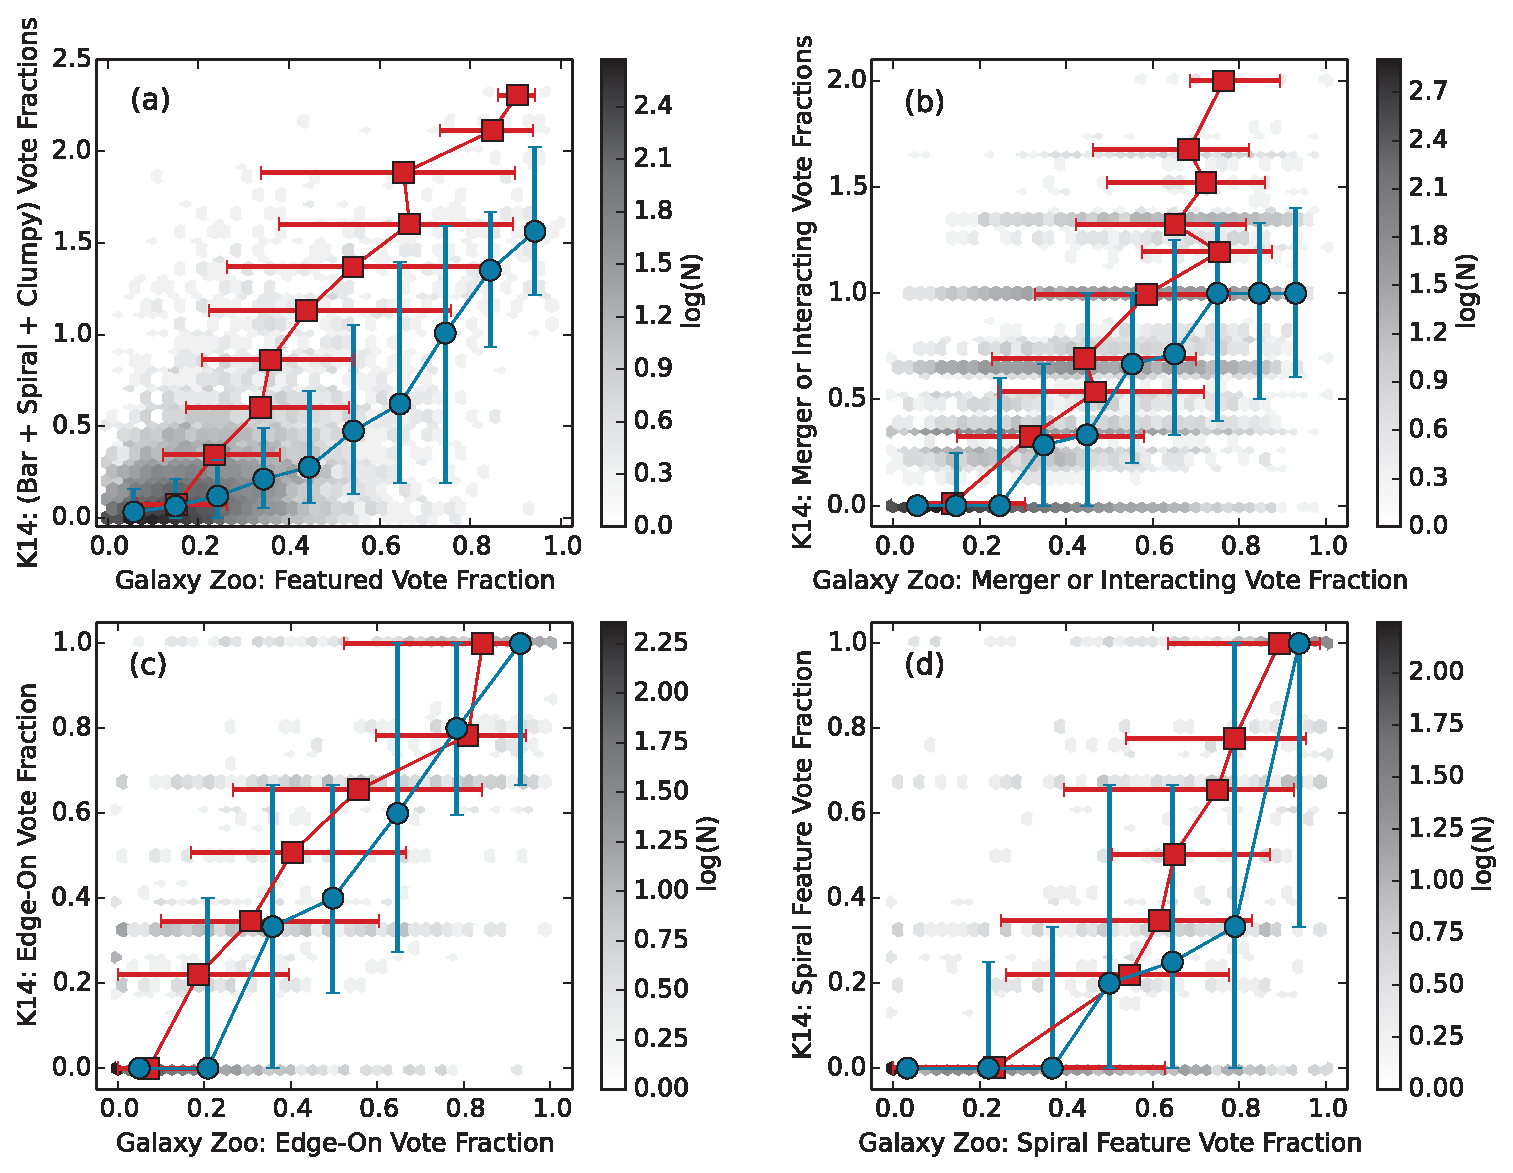
\includegraphics[scale=0.65]{gzteam_candelsteam_multiplot_compareboth.eps}
\caption{
Comparison of Galaxy Zoo classifications with visual classifications from the CANDELS team \citep[][K15]{kartaltepe15}. The classification questions differ between the two projects, but we have selected 4 different classifications which are the most similar: (a) the sum of vote fractions in K15 for spiral, bar, and clumpy features, versus the Galaxy Zoo vote fraction for ``Features or Disk'' in task T00. Note that the sum of these vote fractions from K15 can add to $> 1$; (b) vote fractions for merger or interactions (task T16 in the Galaxy Zoo decision tree) for those subjects not identified as ``Star or Artifact'' in task T00; (c) vote fractions for the presence of an edge-on disk (task T09) for subjects that are neither artifacts nor predominantly smooth, nor dominated by clumps; and (d) vote fractions for the presence of spiral arms (task T12) for those subjects in panel (c) that are not edge-on. In all panels, the number of individual galaxies in a given hexagon in parameter space is shown by its shaded value. Red lines are intended to help guide the eye; the dashed lines show average values within diagonal bins of slopes $\{-2.5, -2, -1, -1\}$ for panels $\{a, b, c, d\}$, and red solid lines show the width of the middle 68 per cent region. The different visual classification methods track each other well across many different kinds of structural classification.
}
\label{fig:candels_compare}
\end{figure*}
%%%%% END FIGURE %%%%%

\subsection{Featured Galaxies}

We seek to compare the overall classification of CANDELS galaxies as ``smooth'' or ``featured'' between Galaxy Zoo and the CANDELS team. However, the team interface described in K15 does not specifically ask about this distinction. It does ask about disks and spheroids; however, equating ``smooth'' to ``spheroid'' and ``featured'' to ``disk'' requires assumptions about galaxies at $z > 1$ that we would prefer to avoid (see Section \ref{sec:result} for a discussion of ``smooth'' disks).

We therefore compare the ``Features or Disk'' vote fraction for T00 in Galaxy Zoo CANDELS to a combination of vote fractions from the CANDELS team classifications. We choose a set of structures that are unambigously inconsistent with a smooth light distribution in a galaxy, namely spiral arms, clumps, and bar features. 

Within the CANDELS team classification interface, a classifier may indicate the presence of a bar or spiral arms by selecting one response for each, $f_{\rm bar, \textsc{ct}}$ or $f_{\rm spiral, \textsc{ct}}$. The clumpy classification, however, is actually a rating of both ``clumpiness'' and ``patchiness'', in a $3 \times 3$ grid with ratings from 0 to 2 along each axis. According to K15, ``Clumps are concentrated independent knots of light while patches are more diffuse structures.'' Both are distinct from a smooth light distribution, so we include both in the creation of a ``featured'' vote for the CANDELS team classifications.

We follow an approach similar to \citet{guo15} in combining clumpy classifications within this matrix of possible responses. Each vote is weighted by the strength of features that it indicates, by assigning a weight of 0.25 for each level along each axis. For a clumpiness rating $i$ and a patchiness rating $j$, the weight for that vote fraction is $$w_{ij} = 0.25 (i + j) .$$ For example, the weight for $C_1 P_2$ = 0.75. As the maximum value within the selection matrix is  $C_2 P_2$, the maximum weight is 1. The overall clumpy vote fraction for a given object is then $$f_{\rm clumpy, \textsc{ct}} = \sum_i{\sum_j{w_{ij} f_{ij}}} .$$ We note that classifiers may make multiple selections within the clumpiness/patchiness rating matrix, so the weighted, summed vote fraction $f_{\rm clumpy}$ can in principle exceed 1.

Figure \ref{fig:candels_compare}a shows the summed ``featured'' vote fraction for the CANDELS team, $f_{\rm bar, \textsc{ct}} + f_{\rm spiral, \textsc{ct}} + f_{\rm clumpy, \textsc{ct}}$, versus the Galaxy Zoo vote fraction for the response ``Features or Disk'' to task T00, for the 13,195 galaxies that have been classified by both and that meet the surface-brightness and other criteria described at the start of Section \ref{sec:comparison}. The figure shows the 2-D histogram via hexagonal shading, indicating that in both projects a high vote for features of any kind is relatively rare (most galaxies have $f_{\rm features} \sim 0$ and $f_{\rm features, \textsc{ct}} \sim 0$). 

The featured vote fractions track each other well, with a clear correlation shown by the red points indicating the average in equal-sized $(x, y)$ bins, a method chosen to show deviations from a linear correlation without favouring either data set as ``correct''. There are virtually no galaxies for which the CANDELS team voted strongly for features being present but the Galaxy Zoo classifiers did not. It is also rare for the Galaxy Zoo classifiers to find a proportionally higher vote fraction for features than the CANDELS team, although the few examples seen in this parameter space may contain examples of distraction bias in a classification interface that presents dozens of choices simultaneously. This is clearly a small effect, however: on the whole the classifications agree very well with each other.
% correlation coefficient 0.5688


\subsection{Merging or Interacting Galaxies}

The last task (T16) in the Galaxy Zoo decision tree asks whether the classifier sees evidence of a merger, or of tidal interaction, or both, or neither. The CANDELS team Interaction Class asks the classifier to decide whether the galaxy is a merger, or whether there is interaction within the segmentation map, or outside of it, with an additional option for a non-interacting companion. There is also a separate flag within the CANDELS team classification to indicate whether a galaxy has tidal arms. Because these selections between projects are similar but not exactly the same, we choose to compare the sum of all signs of interaction of any kind within both projects. Specifically, we consider the sum of vote fractions within the CANDELS team classifications for ``Merger'', ``Interaction within Segmap'',  ``Interaction beyond Segmap'', and ``Tidal Arms'', while for Galaxy Zoo we consider the sum of vote fractions for ``Merger'', ``Tidal Interaction'', or ``Both''. Given this selection, the maximum value for the combined CANDELS team vote is 2, whereas for Galaxy Zoo the maximum vote fraction is 1.

Figure \ref{fig:candels_compare}b compares these fractions for each galaxy in the same way as Figure \ref{fig:candels_compare}a, with darker shaded bins representing a higher number of galaxies within that bin, and with red squares indicating the average binned in both directions. The striations seen in the figure reflect the finite number of possible vote fractions within the CANDELS team votes; this structure was not seen in Figure \ref{fig:candels_compare}a due to the weighted combination of clumpy vote fractions. 

%The majority of subjects received 3 independent classifications each by the CANDELS team, and thus the majority of vote fractions fall within fractions of thirds. We therefore choose asymmetric bins within which to calculate average Galaxy Zoo vote fractions, with the aim of minimising the spread in source counts per bin: bins falling in increments of thirds include only sources with those exact CANDELS team vote fractions, and each bin between those values covers every other value. We adopt this binning strategy in Figures \ref{fig:candels_compare}c and d as well.

Although Galaxy Zoo and the CANDELS team measure different aspects of mergers differently, in combination the merger/interaction vote fractions clearly correlate. As in the comparison between overall featured fractions, there are more examples where the Galaxy Zoo vote fraction is notably higher than the CANDELS team vote fraction than vice-versa. Examination of galaxies where Galaxy Zoo $f_{\rm merger\ or\ interaction} > 0.5$ and CANDELS team $f_{\rm merger\ or\ interaction, \textsc{ct}} = 0$ indicates some cases where a merger or tidal feature is clearly present, but others where it is less obvious whether a nearby companion is interacting. 

Indeed, among this sample the CANDELS team vote fraction for ``Non-Interacting Companion'' is considerably higher on average than for the overall sample. This option is not explicitly available to Galaxy Zoo classifiers, although even moderately experienced classifiers, particularly those who participate in discussions within the community Talk software, will in general select ``Neither'' if they decide the companion is not interacting. This explains why the number of galaxies showing this mismatch is much smaller (less than 2\% of the sample) than the overall number of galaxies which CANDELS team classifications mark as having a non-interacting companion. Future analyses of mergers and interacting galaxies may find a combination of Galaxy Zoo and CANDELS team classifications useful for eliminating the effects of distraction bias and distinguishing between interacting and non-interacting companions.

% correlation coefficient 0.6645

\subsection{Edge-On Galaxies}

As described in Section \ref{sec:usage}, the branched nature of the Galaxy Zoo decision tree means that selecting a sample for comparison of edge-on vote fraction requires care. We thus consider, in addition to the previous sample requirements, that a galaxy must also have a featured vote fraction $f_{\rm features} \geq 0.3$ and a not-clumpy vote fraction $f_{\rm not\ clumpy} \geq 0.3$. This selection favours completeness over purity, and is thus appropriate for a comparison of different visual classification methods. The selection results in a sample of 1,273 galaxies.

Both the CANDELS team and Galaxy Zoo classifications allow for the flagging of a galaxy as edge-on with a single selection, allowing for direct comparison. Figure \ref{fig:candels_compare}c shows the CANDELS team versus the Galaxy Zoo classification vote fractions. The two agree very well, with the average vote fraction generally consistent with a 1:1 line. 

% correlation coefficient 0.8069

\subsection{Spiral Galaxies}

The spiral galaxy tasks in Galaxy Zoo are 1 branch below the edge-on disk galaxy task (T09), introducing another dependency on the sample selection, as described in Section \ref{sec:usage}. From within the sample used to construct Figure \ref{fig:candels_compare}c, we further require a vote of $f_{\rm not\ edge-on} \geq 0.5$, a selection chosen to balance the desire for completeness with the need to be able to see spiral arms if they are present. This selects 941 galaxies, whose positions in Figure \ref{fig:candels_compare}d are shown in the 2-D shaded histograms. 

As in all other morphological parameters shown in Figure \ref{fig:candels_compare}, the visual classifications from both projects agree very well. Outliers in this figure include some examples that are best explained by distraction bias in the absence of a decision tree in CANDELS, and also include a few examples of distraction bias of a different sort in Galaxy Zoo: a handful of subjects that include a spiral galaxy very near the central, much fainter, galaxy. Such examples are a very small part of the overall sample, and are relatively easily rejected from a sample selection in any case. In general the classifications agree very well along this and other morphological axes which are directly comparable between the CANDELS team and Galaxy Zoo visual classifiations.


% correlation coefficient 0.5676





%%%%%%%%%%%%%%%%%%%%%%%%%%%%%%%%%%%%%%%%%%%%%%
%
%  
\section{A population of ``smooth'' disk galaxies}\label{sec:result}
%
%
%%%%%%%%%%%%%%%%%%%%%%%%%%%%%%%%%%%%%%%%%%%%%%


Although the morphological classifications described here present quantified visual assessments of a range of galaxy properties, the classification tree described in Section \ref{sec:tree} never explicitly asks the classifier to decide whether a galaxy has a disk. While many questions ask about disk instability features, there is no attempt to identify disks. This choice of what \emph{not} to ask, which echoes that of previous Galaxy Zoo projects, partly reflects a discomfort with asking classifiers to assess light concentrations by eye without any further context. 

Thus within the Galaxy Zoo CANDELS classifications disks may be identified by the presence of specific features, but the absence of these features does not necessarily imply the lack of a disk, particularly at the epochs probed here. Decoupling questions about ``features'' from measures of a galaxy's diskiness enables these to be assessed independently. Specifically, while galaxies with strong ``features'' (as defined by the classification tree in Section \ref{sec:tree}) may be prone to systematic biases in identification of disks via \citet{sersic68} index measurements, galaxies which are more ``smooth'' do not suffer from these effects, and thus disk strength may be more accurately assessed. With the advent of new tools to measure light profiles via simultaneous consideration of multi-wavelength imaging \citep{haeussler13}, measurements of relative bulge and disk strengths are now possible with much higher accuracy than available for single-wavelength measurements at $z \sim 2$. 

To compare the Galaxy Zoo classifications of ``Featured'' and ``Smooth'' to measurements of disk strength, we first select samples of Smooth and of Featured galaxies by selecting subjects with redshifts $1 \leq z \leq 3$, with surface brightnesses brighter than 24.5 mag~arcsec$^{-2}$, and which have ``Star or Artifact'' vote fractions (as described in Section \ref{sec:release}, from the {\small \tt t00\_smooth\_or\_featured\_a2\_artifact\_weighted\_frac} column) $f_{\rm artifact} < 0.4$. For the Smooth sample, we select galaxies having $f_{\rm smooth} \geq 0.6$; galaxies in the Featured sample have $f_{\rm features} \geq 0.6$.

Each sample is further refined by matching to multi-wavelength $IJH$ bulge-disk decompositions of galaxies in the CANDELS fields by Haeussler et al. (in preparation) using the software package MegaMorph \citep{haeussler13}. We choose galaxies where the bulge-disk fits reported no error flags and where the fit parameters converged to values well within the limits of constraints set by the fitting routine (i.e., limits on S\'ersic index and effective radius of $0.22 \leq n \leq 7.8$ and $0.33 \leq r_e \leq 390$, respectively). These selections result in a sample of 72 Featured galaxies and 1117 Smooth galaxies with reliable bulge-disk decompositions.

Figure \ref{fig:btot} shows the distribution of bulge-to-total luminosity ratio (flux-summed to obtain one measurement across $IJH$) in the Featured and Smooth samples. A Kolmogorov-Smirnov test indicates the B/Tot distributions of Smooth and Featured galaxies are inconsistent with being drawn from the same parent sample at the $5 \sigma$ significance level. As expected, Featured galaxies are generally disk-dominated. However, the Smooth galaxies have a considerably more uniform distribution of bulge-to-total ratios, such that 25\% of galaxies in the Smooth sample have disk-dominated light profiles (B/Tot~$\leq 0.25$). 

This finding of a substantial population of completely smooth disk galaxies is consistent with the results of recent dynamical studies of galaxies at $z > 1$ \citep[e.g.][]{wisnioski15}. Moreover, because galaxies with smoother light distribution are also more likely to have very reliable bulge-disk decompositions in large-scale galaxy fitting studies, the combination of Galaxy Zoo morphological selection and selection of smooth disks via bulge-to-total ratios is a more powerful selector of relatively complete samples of $z > 1$ disks than either selection method alone.

%%%%% [FIGURE: BTot] %%%%%
\begin{figure}
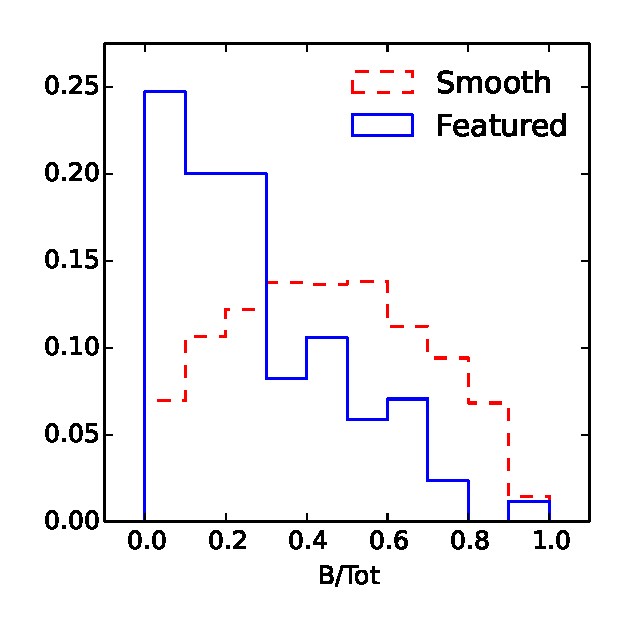
\includegraphics[scale=0.85]{BTot_histogram.eps}
\caption{
Distributions of bulge-to-total ratios for samples of galaxies that are unambiguously Smooth (red dashed histogram) and Featured (blue solid histogram). The majority of features measured by Galaxy Zoo CANDELS are associated with disk instabilities; thus it is perhaps not surprising that the Featured sample is generally disk-dominated. However, the Smooth galaxy sample has a relatively uniform distribution of bulge-to-total ratios, including a substantial population of disk-dominated galaxies at $1 \leq z \leq 3$ which have no evidence of significant features.
}
\label{fig:btot}
\end{figure}
%%%%% END FIGURE %%%%%




%%%%%%%%%%%%%%%%%%%%%%%%%%%%%%%%%%%%%%%%%%%%%%
%
%  
\section{Summary}\label{sec:summary}
%
%
%%%%%%%%%%%%%%%%%%%%%%%%%%%%%%%%%%%%%%%%%%%%%%

The Galaxy Zoo project has collected typically 40 or more independent visual classifications to date from colour images of 3 CANDELS fields: GOODS-South, COSMOS, and the UDS. Here we present the public release of these classifications, after applying an iterative consensus-based classifier weighting scheme that has been successfully applied to multiple previous Galaxy Zoo projects, as well as additional weighting techniques making use of the stellarity parameter from automated measurements. We provide an analysis of changes in classifications with imaging depth and offer caveats and advice for usage of these morphological measurements for different science goals. 

Comparison of the Galaxy Zoo morphologies with existing visual morphologies of a subset of the sample are in excellent agreement across a wide range of morphological features. We also combine Galaxy Zoo morphologies with multi-wavelength bulge-disk decompositions to show that a substantial fraction of galaxies lacking significant morphological signatures of disk features have disk-dominated light profiles.

The public catalog of Galaxy Zoo CANDELS morphologies may be obtained from {\tt data.galaxyzoo.org}.
  
%%%%%%%%%%%%%%%%%%%%%%%%%%%%%%%%%%%%%%%%%%%%%%
%%%%%%%%%%%%%%%%%%%%%%%%%%%%%%%%%%%%%%%%%%%%%%
%%%%%%%%%%%%%%%%%%%%%%%%%%%%%%%%%%%%%%%%%%%%%%
%%%%%%%%%%%%%%%%%%%%%%%%%%%%%%%%%%%%%%%%%%%%%%
%
%
\section*{Acknowledgments}
%
%
%%%%%%%%%%%%%%%%%%%%%%%%%%%%%%%%%%%%%%%%%%%%%%

%TOPCAT \citep{taylor05} and an OS X widget form of the JavaScript Cosmology Calculator \citep{wright06} were used while preparing this paper. 
%
%BDS gratefully acknowledges support from the Oxford Martin School, Worcester College and Balliol College, Oxford.
%
%TM acknowledges funding from the Science and Technology Facilities Council ST/J500665/1.
%
%KLM acknowledges funding from The Leverhulme Trust as a 2010 Early Career Fellow.
%
%KWW and LF acknowledge funding from the UMN Grant-In-Aid program. 
%
%RCN acknowledges STFC Rolling Grant ST/I001204/1 to ICG for �Survey Cosmology and Astrophysics�. 
%
%KS gratefully acknowledges support from Swiss National Science Foundation Grant PP00P2\_138979/1. 
%

The development of Galaxy Zoo was supported in part by the Alfred P. Sloan Foundation. Galaxy Zoo was supported by The Leverhulme Trust. 

This work is based on observations taken by the CANDELS Multi-Cycle Treasury Program with the NASA/ESA HST, which is operated by the Association of Universities for Research in Astronomy, Inc., under NASA contract NAS5-26555.
  
\bibliographystyle{mn2e}
\bibliography{refs}  


  
\end{document}
  
